\chapter{Research Results}\label{chap:research_results}

This section examines prototype testing results, comparing Thread network performance in various modes and locations to assess the effectiveness of the Monte Carlo Method and Genetic Algorithm optimization in enhancing energy efficiency.

\section{Algorithm Output}\label{sec:algorithm_output}
This subsection investigates the output from Monte Carlo and Genetic Algorithm simulations, which are crucial in determining transmission power settings for the Thread network.

\subsection{Monte Carlo Method}\label{sec:monte_carlo_method_output}
The parameters table \ref{tab:mcm_parameters} provides insights into network performance based on transmission power values derived from the Monte Carlo Method. These parameters greatly influence results, making the table essential for comprehending the context of the generated output. Since the research was conducted in two distinct locations, it is necessary to showcase the Monte Carlo Method outputs separately for each location.

\subsubsection{Location: Lab}\label{sec:monte_carlo_method_output_lab}
This section presents the Monte Carlo Method output for the Lab location. The table below shows a few network configuration rows generated by the method, with thousands in total. Space limitations restrict the display to the last rows. The final row represents the correct configuration without penalty, meeting the mathematical model for appropriate device types and initial transmission powers.

\begin{longtblr}[
  caption = {Monte Carlo Method output from Lab.},
  label = {tab:monte_carlo_method_output_lab},
  ]{
  colspec = {X[l] X[l] X[l] X[l] X[l] X[l]},
  hlines, vlines,
  rowhead = 1, % Repeat the header row on every page
  row{1} = {font=\bfseries},
}
  Device Type & txpower & Total txpower & Penalty & RSSI Penalty & Entire Power \\
  3, 5, 2, 5, 1, 5, 0, 0 & -20, 0, 0, -8, 0, -12, 0, -20 & -60 & 3000 & 0 & 2940 \\
  3, 4, 1, 3, 0, 4, 1, 3 & -16, -8, -4, -20, 0, -12, -4, -20 & -84 & 3000 & 0 & 2916 \\
  3, 4, 4, 1, 2, 4, 4, 2 & 4, -12, -20, -4, -8, -12, -20, -8 & -80 & 3000 & 0 & 2920 \\
  2, 0, 1, 2, 0, 0, 1, 1 & -12, 4, -8, -8, -20, 0, -8, -20 & -72 & 4000 & 0 & 3928 \\
  2, 5, 3, 3, 5, 2, 2, 4 & -8, 8, 0, -16, 0, -8, -20, 8 & 36 & 0 & 0 & 36 \\
\end{longtblr}


Additionally, Monte Carlo Method generates a comprehensive table with details on each device in the network configuration, including individual distances, path loss, RSSI for downlink and uplink, and sensitivity penalties. Due to its size, we present only the first five rows of the correct configuration output. Examining these selected outputs offers insights into network performance and efficiency in each environment, keeping the focus on the primary research objectives.

\begin{longtblr}[
  caption = {Device specific output from Monte Carlo Method for Lab.},
  label = {tab:monte_carlo_method_output_lab_device_specific},
  ]{
  colspec = {X[l] X[l] X[l] X[l] X[l] X[l] X[l]},
  hlines, vlines,
  rowhead = 1, % Repeat the header row on every page
  row{1} = {font=\bfseries},
}
  Current Device & Next Device & Distance & Path Loss & RSSI Downlink & RSSI Uplink & Sensitivity Penalty \\
  5 & 5 & 0.00 & 2.08 & 7.91 & -0.08 & 0 \\
  5 & 4 & 0.15 & -0.02 & 10.02 & 10.02 & 0 \\
  5 & 3 & 1.50 & -9.06 & -19.06 & 11.06 & 0 \\
  5 & 3 & 1.50 & -12.55 & 22.55 & -1.44 & 0 \\
  5 & 2 & 2.30 & -9.85 & 19.85 & 3.85 & 0 \\
\end{longtblr}


\subsubsection{Location: Home}\label{sec:monte_carlo_method_output_home}
Similarly, this section focuses on the Monte Carlo Method output for the Home location. The table below displays several rows of the network configuration data from the Monte Carlo Method for the home location. The last row in the table represents the correct configuration that has no penalty and satisfies the mathematical model.

\begin{longtblr}[
  caption = {Monte Carlo Method output from Home.},
  label = {tab:monte_carlo_method_output_home},
  ]{
  colspec = {X[l] X[l] X[l] X[l] X[l] X[l]},
  hlines, vlines,
  rowhead = 1, % Repeat the header row on every page
  row{1} = {font=\bfseries},
}
  Device Type & txpower & Total txpower & Penalty & RSSI Penalty & Entire Power \\
  2, 0, 2, 2, 5, 5, 1, 1 & -12, -8, 8, -4, 0, 8, -20, -12 & -40 & 3000 & 0 & 2960 \\
  4, 1, 1, 4, 0, 5, 1, 0 & -12, 4, 0, -8, 8, 8, -12, -20 & -32 & 4000 & 0 & 3968 \\
  0, 2, 5, 2, 4, 2, 5, 4 & -20, -4, -12, -12, -4, -8, -20, -4 & -84 & 3000 & 0 & 2916 \\
  1, 2, 0, 2, 1, 2, 0, 1 & -8, -8, -16, -16, -12, -8, -16, 4 & -80 & 4000 & 0 & 3920 \\
  2, 3, 5, 2, 2, 3, 4, 5 & 8, 8, -20, -8, -4, -16, 4, -16 & -44 & 0 & 0 & -44 \\
\end{longtblr}

Moreover, the following table represents some of the comprehensive data for specific devices. By analyzing this table, we can understand the inter-device relationships and the factors impacting the overall performance of the wireless communication network at the home location. This detailed information is valuable in identifying potential areas for improvement and optimization.

\begin{longtblr}[
  caption = {Device specific output from Monte Carlo Method for Home.},
  label = {tab:monte_carlo_method_output_home_device_specific},
  ]{
  colspec = {X[l] X[l] X[l] X[l] X[l] X[l]},
  hlines, vlines,
  rowhead = 1, % Repeat the header row on every page
  row{1} = {font=\bfseries},
}
  Current Device & Next Device & Distance & Path Loss & RSSI Downlink & RSSI Uplink & Sensitivity Penalty \\
  5 & 5 & 0.00 & 34.99 & -52.99 & -48.99 & 0 \\
  5 & 4 & 5.00 & 32.08 & -50.08 & -26.08 & 0 \\
  5 & 3 & 10.00 & 14.02 & -32.02 & -4.02 & 0 \\
  5 & 3 & 10.00 & 28.33 & -46.33 & -42.33 & 0 \\
  5 & 2 & 15.00 & 23.05 & -41.05 & -13.05 & 0 \\
\end{longtblr}


A comparison between the lab and home locations reveals some key differences. With its smaller room size, the lab location experiences lower path loss and RSSI values, attributed to more efficient signal transmission. In contrast, the home location exhibits higher path loss and RSSI values due to the increased distance between devices. By analyzing these outputs, we can better understand the impact of various environments and distances on network performance, allowing for informed optimization decisions for different applications.


\section{Genetic Algorithm}\label{sec:genetic_algorithm_output}
This section highlights the Genetic Algorithm output and key parameters affecting the results. The parameters in table \ref{tab:ga_parameters} are crucial as they significantly influence outcomes. The GA algorithm was applied in lab and home settings, with outputs presented separately for comparison and analysis under different environmental conditions. This approach provides insight into the GA algorithm's performance and adaptability in optimizing wireless communication networks across various scenarios.


\subsubsection{Location: Lab}
This section examines the Genetic Algorithm output for the lab location, highlighting transmission power results. These findings reveal the GA's effectiveness in optimizing power consumption in a lab environment.

\paragraph{Transmission Power}
The power optimization plot demonstrates the effectiveness of the GA in optimizing the transmission power for the devices in the lab. Initially, the maximum transmission power was 56, optimized to the lowest value of -160. This significant reduction in power consumption is expected due to the proximity of the devices in the lab setting, indicating that using the lowest transmission power for each device is the most efficient strategy under these conditions.

\begin{figure}[h]
  \centering
  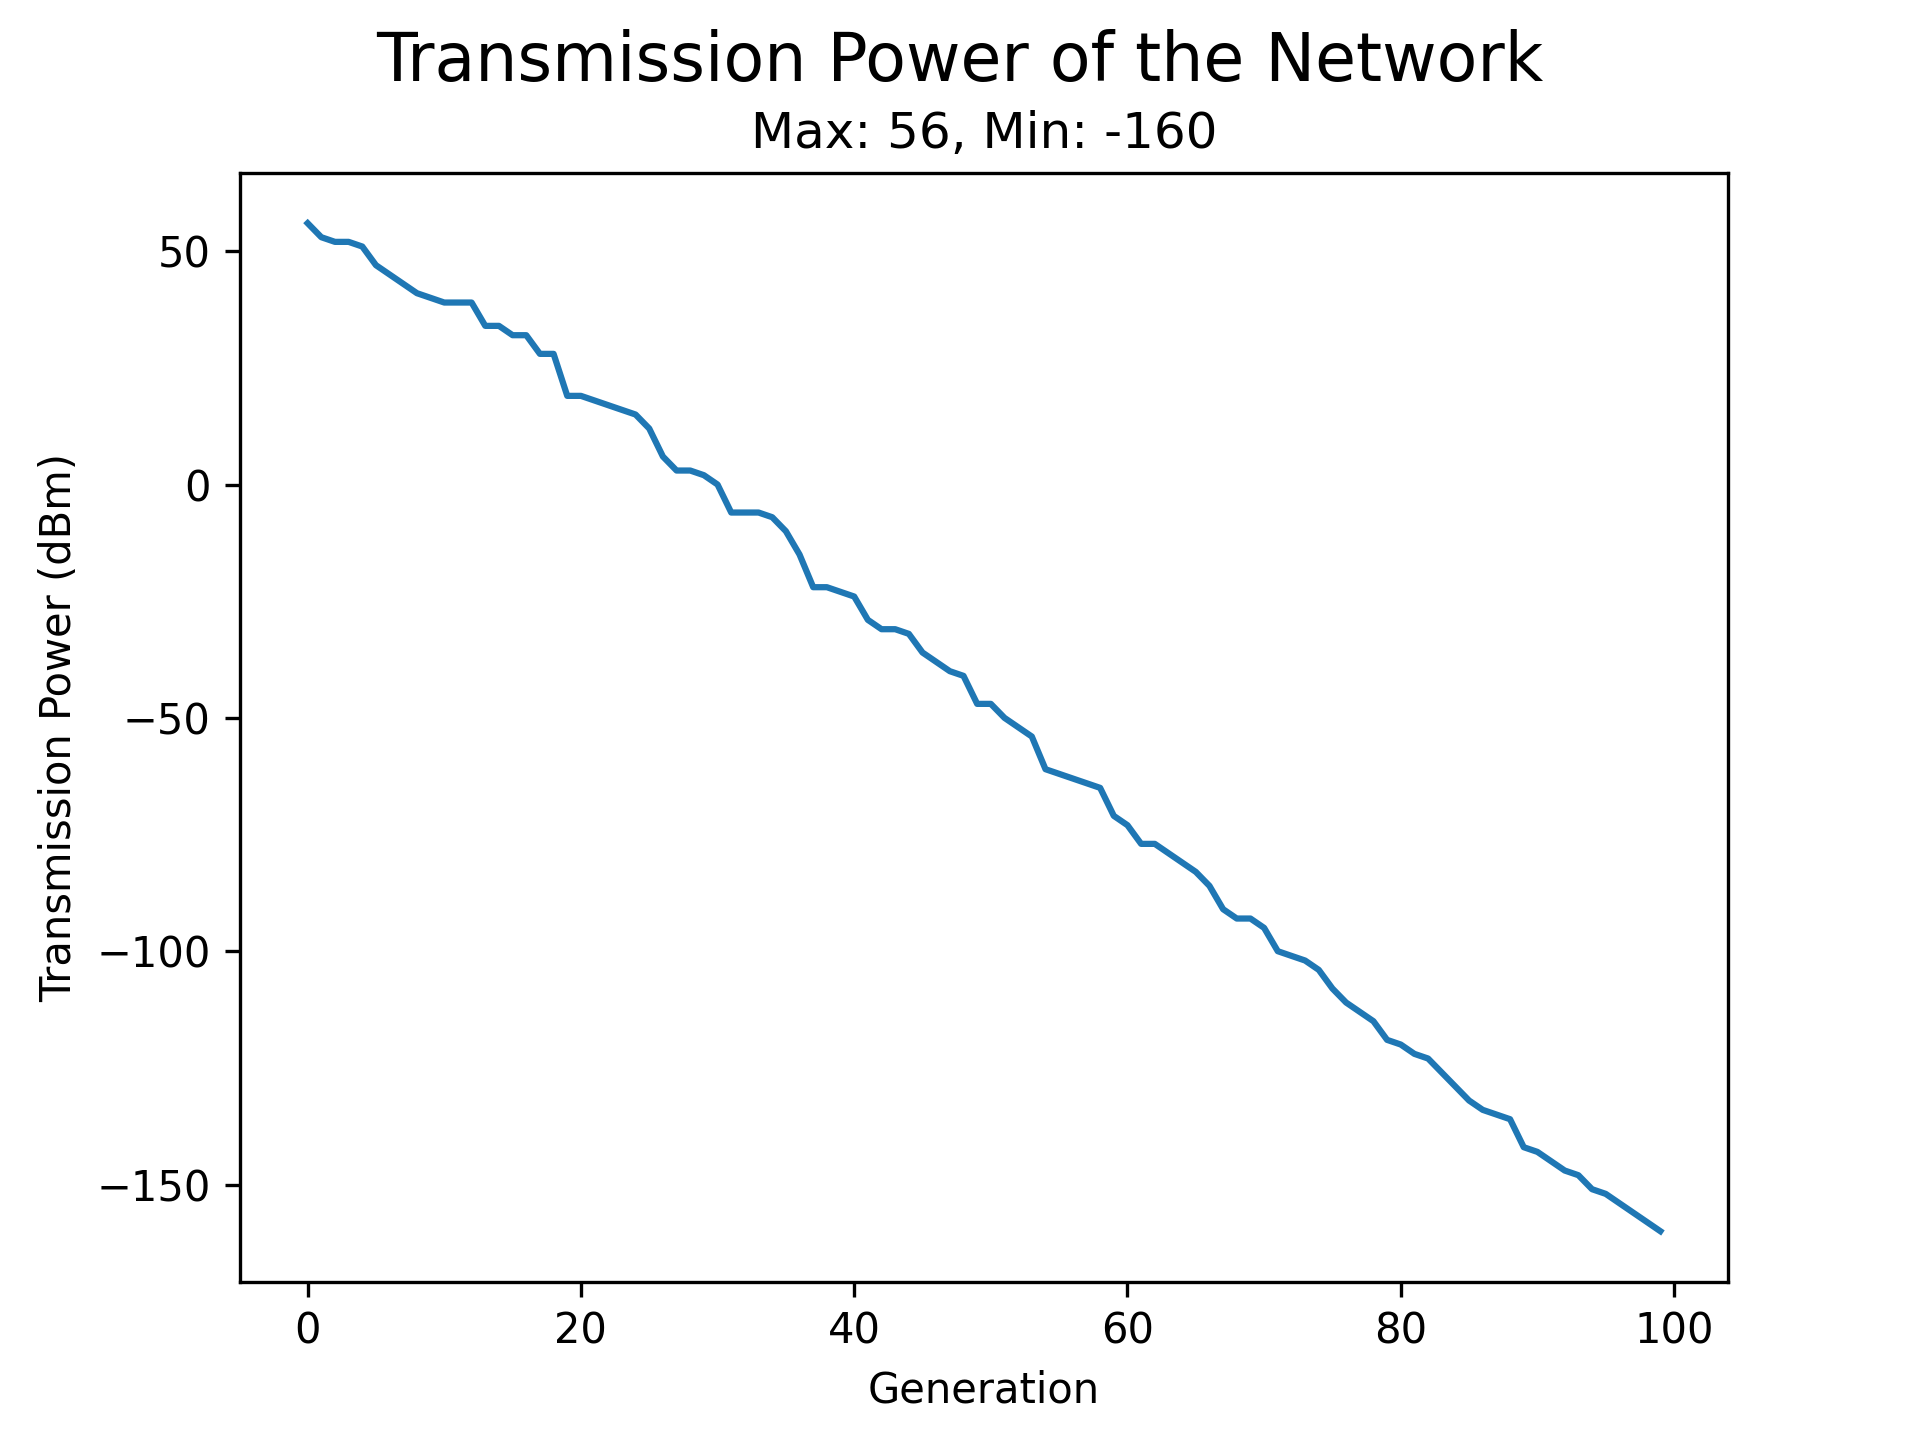
\includegraphics[width=0.5\textwidth]{images/research_results/genetic_algorithm_lab_power.png}
    \caption{Genetic Algorithm transmission power optimization for lab location.}
    \label{fig:genetic_algorithm_lab_power}
\end{figure}

\paragraph{Network Configuration}
The network configuration data obtained from the GA provides information on the list of transmission power, total transmission power, and the maximum transmission power determined by the algorithm. By analyzing these values, we can better understand the factors contributing to an efficient and effective wireless communication network in the lab environment.

\begin{longtblr}[
  caption = {Genetic Algorithm output for lab location.},
  label = {tab:genetic_algorithm_output_lab},
  ]{
  colspec = {X[l] X[l] X[l] X[l] X[l] X[l]},
  hlines, vlines,
  rowhead = 1, % Repeat the header row on every page
  row{1} = {font=\bfseries},
}
  Transmission Power $(dBm)$ & Total $(dBm)$ & Maximum $(dBm)$ \\
  -20, -20, -20, -20, -20, -20, -20, -20 & -160 & 56 \\
\end{longtblr}

\subsubsection{Location: Home}
This section examines the Genetic Algorithm output for the home location, highlighting transmission power. This finding reveals the GA's effectiveness in optimizing power consumption in a home environment.

\paragraph{Transmission Power}
The power optimization plot demonstrates the effectiveness of the GA in optimizing the transmission power for the devices in the home. Initially, the maximum transmission power was 56, optimized to a significantly lower value of -149. This notable reduction in power consumption can be attributed to the GA's ability to adapt the transmission power according to the specific requirements of the home environment, where distances between devices can vary significantly compared to a lab setting.

\begin{figure}[h]
  \centering
  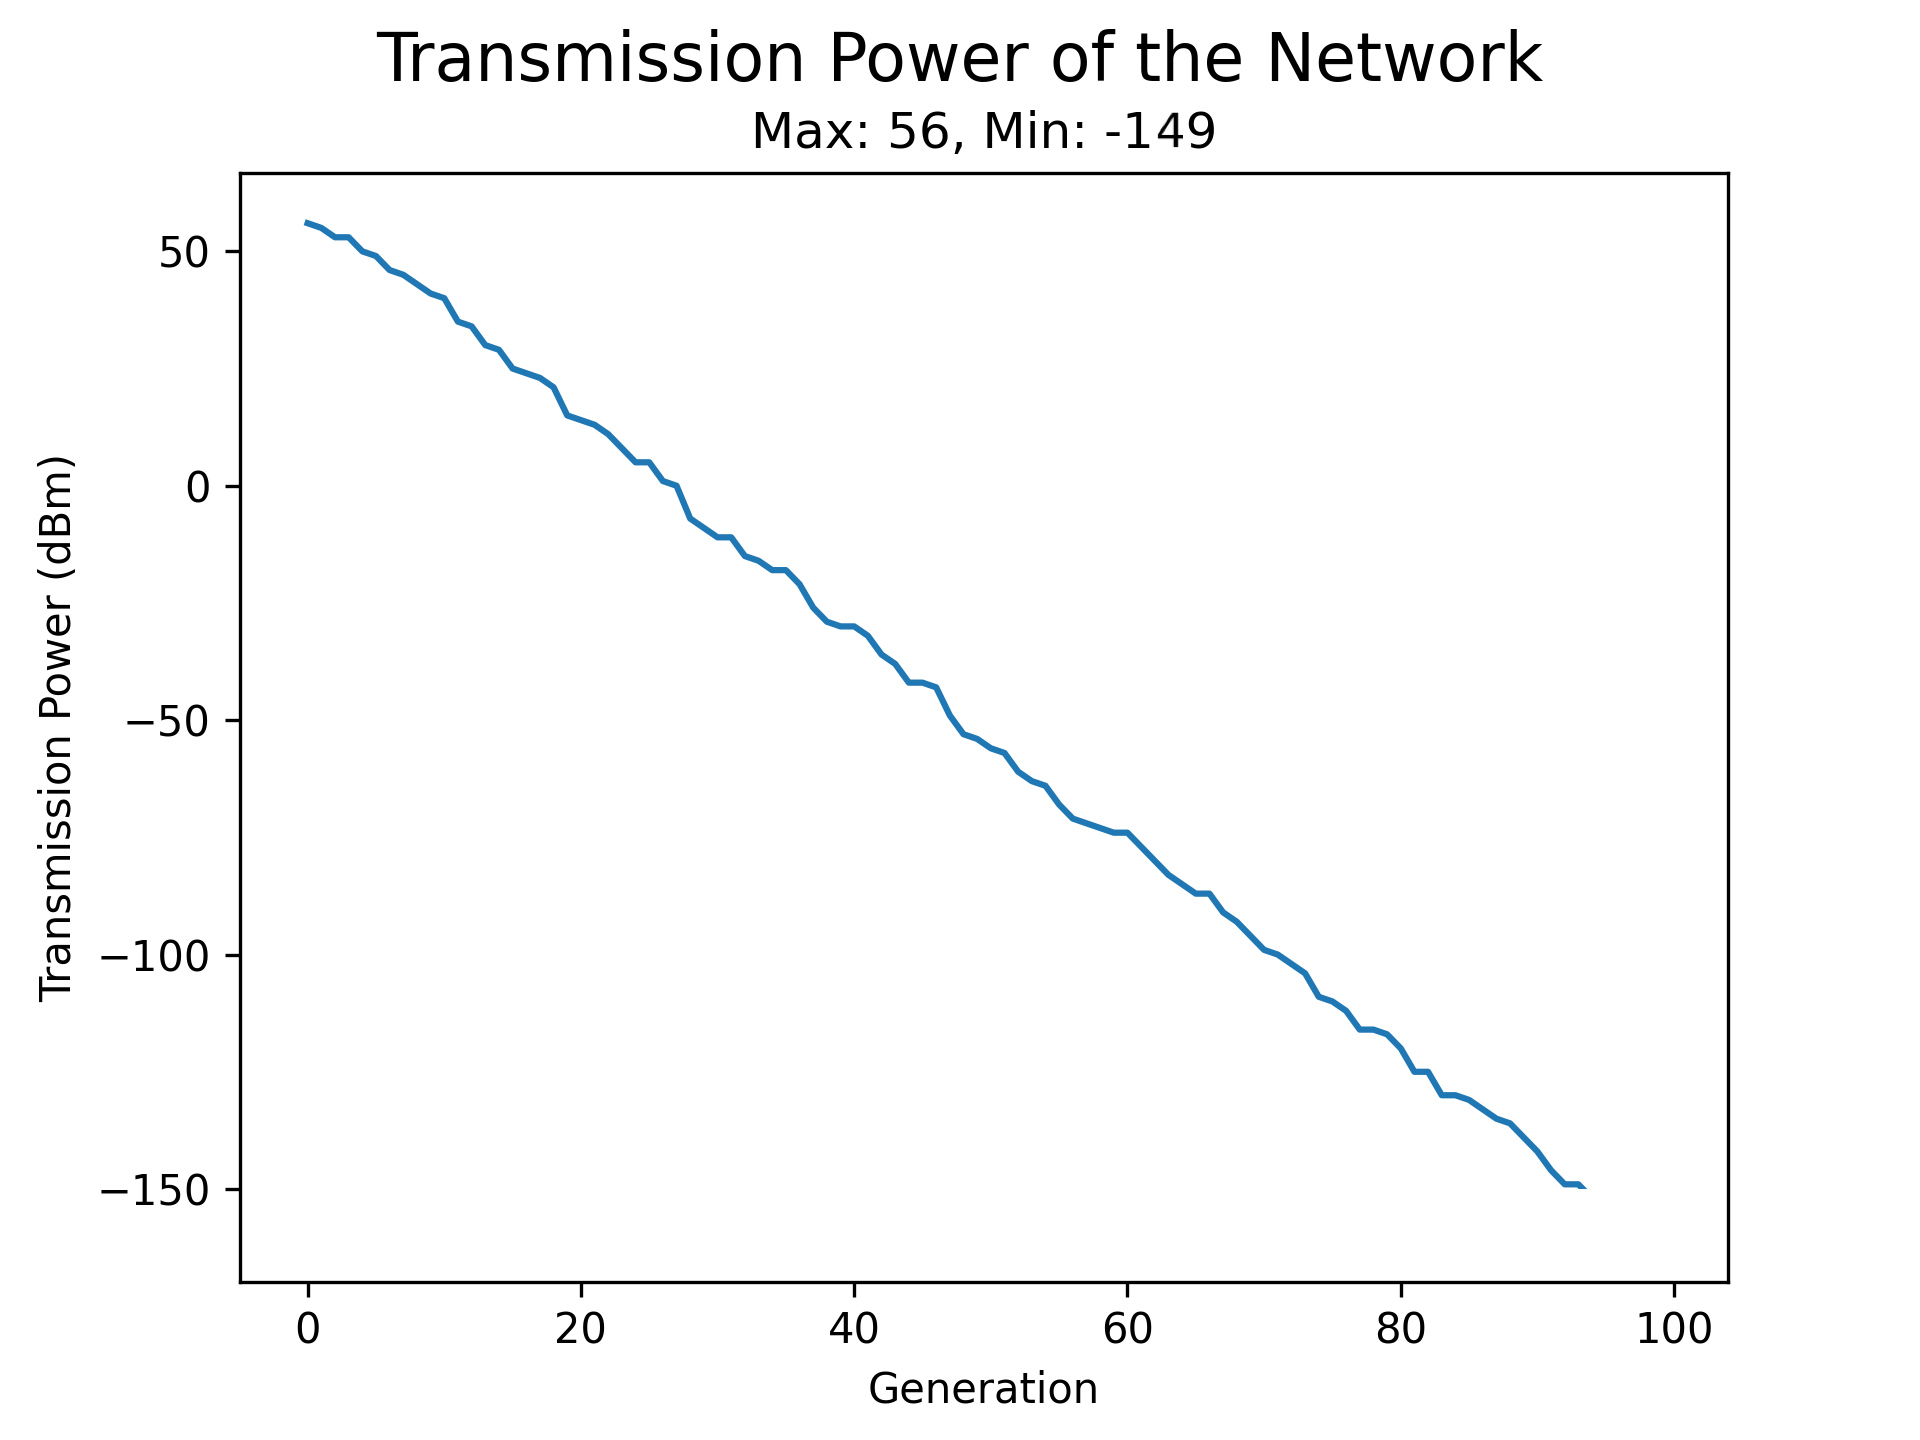
\includegraphics[width=0.5\textwidth]{images/research_results/genetic_algorithm_home_power.png}
    \caption{Genetic Algorithm transmission power optimization for home location.}
    \label{fig:genetic_algorithm_home_power}
\end{figure}

\paragraph{Network Configuration}
Similarly, the network configuration differs from the one observed in the lab setting, highlighting the unique requirements of each environment. In the home location, the devices have a different distribution of transmission power levels to optimize power consumption and maintain efficient communication in the presence of various obstacles and more considerable distances between devices. By adjusting the transmission power according to the specific conditions of the home environment, the GA can find a practical solution that balances power consumption and network performance.

\begin{longtblr}[
  caption = {Genetic Algorithm output for home location.},
  label = {tab:genetic_algorithm_output_home},
  ]{
  colspec = {X[l] X[l] X[l] X[l] X[l] X[l]},
  hlines, vlines,
  rowhead = 1, % Repeat the header row on every page
  row{1} = {font=\bfseries},
}
  Transmission Power $(dBm)$ & Total $(dBm)$ & Maximum $(dBm)$ \\
  -20, -19, -20, -19, -18, -18, -16, -19 & -149 & 56 \\
\end{longtblr}

\subsubsection{Large Random Distance}
In this section, the performance of the GA algorithm, when applied to a considerable distance scenario, is explored. The significant distance output has yet to be tested on the physical prototype due to resource constraints and the impracticality of implementing such a large-scale test. In this scenario, the distance between each device is set to 500 meters apart from one.

\paragraph{Transmission Power}
When observing the transmission power plot for this considerable distance scenario, we find that the GA algorithm can significantly optimize the transmission power from an initial value of 38,877 down to -68 dBm. This impressive optimization result highlights the capability of the GA algorithm to effectively adjust the transmission power even in situations with considerable distances between devices.

\begin{figure}[h]
  \centering
  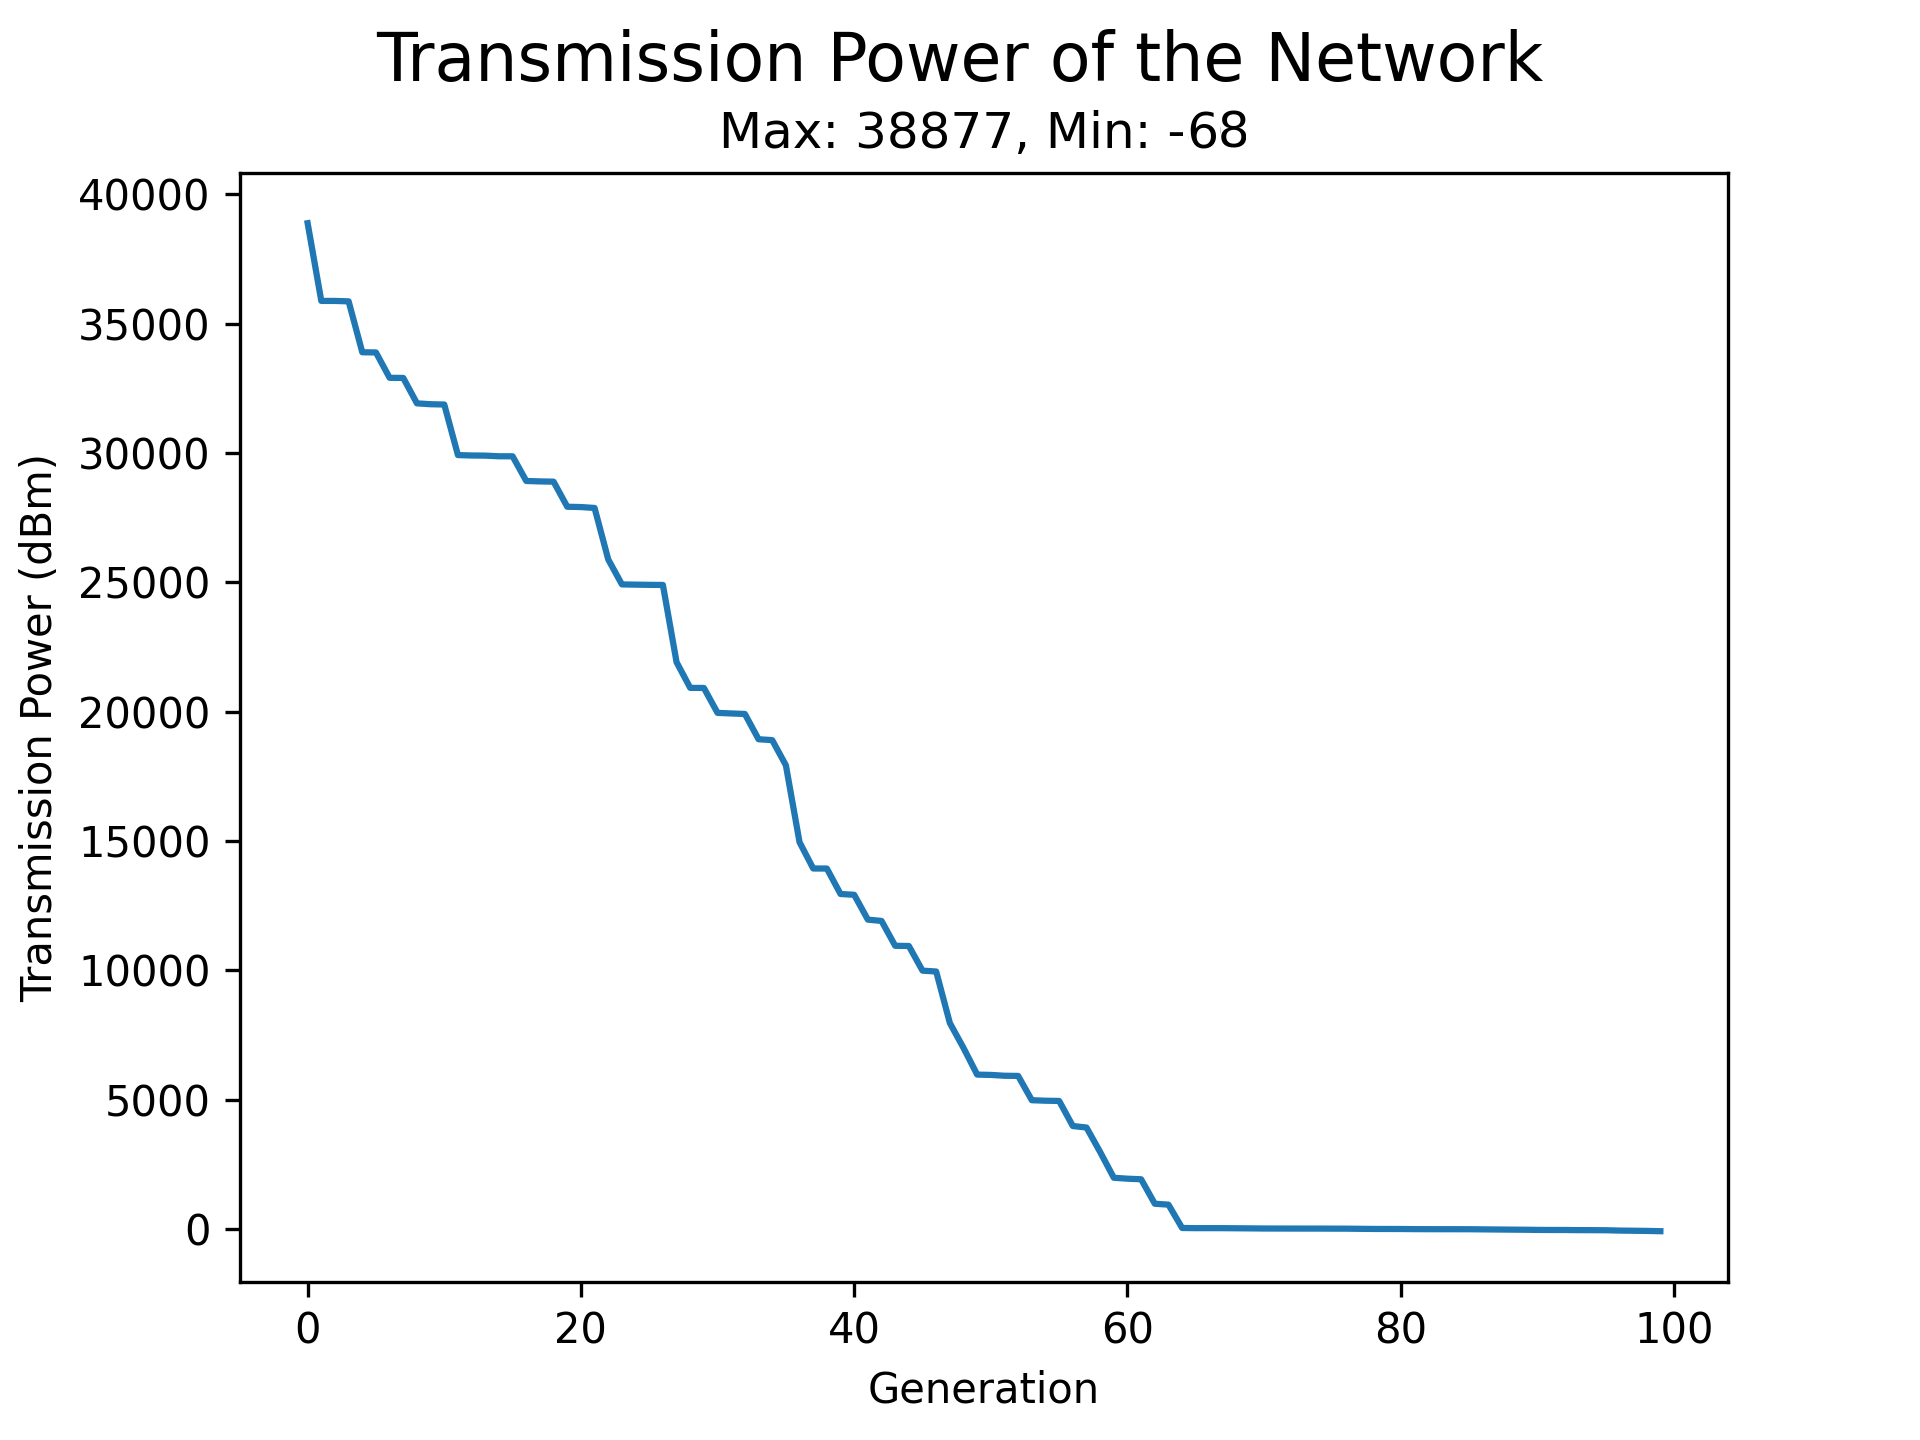
\includegraphics[width=0.5\textwidth]{images/research_results/genetic_algorithm_large_random_distance_power.png}
    \caption{Genetic Algorithm transmission power optimization for large random distance scenario.}
    \label{fig:genetic_algorithm_large_random_distance_power}
\end{figure}

\paragraph{Network Configuration}
In the network configuration for the large distance scenario, the transmission power for each device is no longer set to closer to the lowest value, resulting in a total transmission power of -68 and a maximum value of 38,877. The results from this test demonstrate the potential of the GA algorithm to optimize transmission power over large distances, making it a valuable tool for optimizing wireless communication networks in various environments.

\begin{longtblr}[
  caption = {Genetic Algorithm output for large random distance scenario.},
  label = {tab:genetic_algorithm_output_large_random_distance},
  ]{
  colspec = {X[l] X[l] X[l] X[l] X[l] X[l]},
  hlines, vlines,
  rowhead = 1, % Repeat the header row on every page
  row{1} = {font=\bfseries},
}
  Transmission Power $(dBm)$ & Total $(dBm)$ & Maximum $(dBm)$ \\
  -17, -8, -5, 7, -13, -11, -9, -12 & -68 & 38,877 \\
\end{longtblr}

\subsection{Comparison Overview}
In conclusion, the GA and Monte Carlo algorithms were applied to various scenarios, including large distances, home environments, and laboratory settings, to optimize transmission power in wireless communication networks. However, the GA algorithm stands out for its exceptional ability to optimize transmission power across all scenarios.

In the large distance scenario, the GA algorithm optimized transmission power from a maximum of 38,877 to a minimum of -68, showcasing its remarkable performance in tackling large-scale challenges. In the home and lab environments, the GA algorithm effectively adapted to the specific requirements of these scenarios, optimizing transmission power to -149 and -160, respectively.

While the Monte Carlo algorithm also demonstrated its capacity to optimize transmission power in home and lab settings, the GA algorithm consistently outperformed Monte Carlo in optimizing transmission power across all considered environments.


\section{Current Consumption Analysis}
This section will analyze the current consumption for individual devices in the wireless communication network. We will examine the maximum and optimized current consumption across Lab and Home locations, considering scenarios with and without sensor data and utilizing Monte Carlo Method and Genetic Algorithm optimization.

\subsection{Maximum Current Consumption}
This section investigates the power consumption profiles of devices operating at their highest transmission power setting of 8 dBm, regardless of location and type. This analysis provides a baseline for understanding power consumption limits and identifying potential optimization areas.

\subsubsection{Location: Lab}
This section examines the current consumption at the lab location, a small research room with efficient signal transmission. We discuss the impact of this confined environment on network performance and optimizations, considering the unique characteristics of the lab setting.

\paragraph{Mode: No Sensor}
The following plot and table present an overview of the network's current consumption in No Sensor mode, where devices do not send any pings to their radios, resulting in lower power consumption.

\begin{figure}[H]
  \centering
  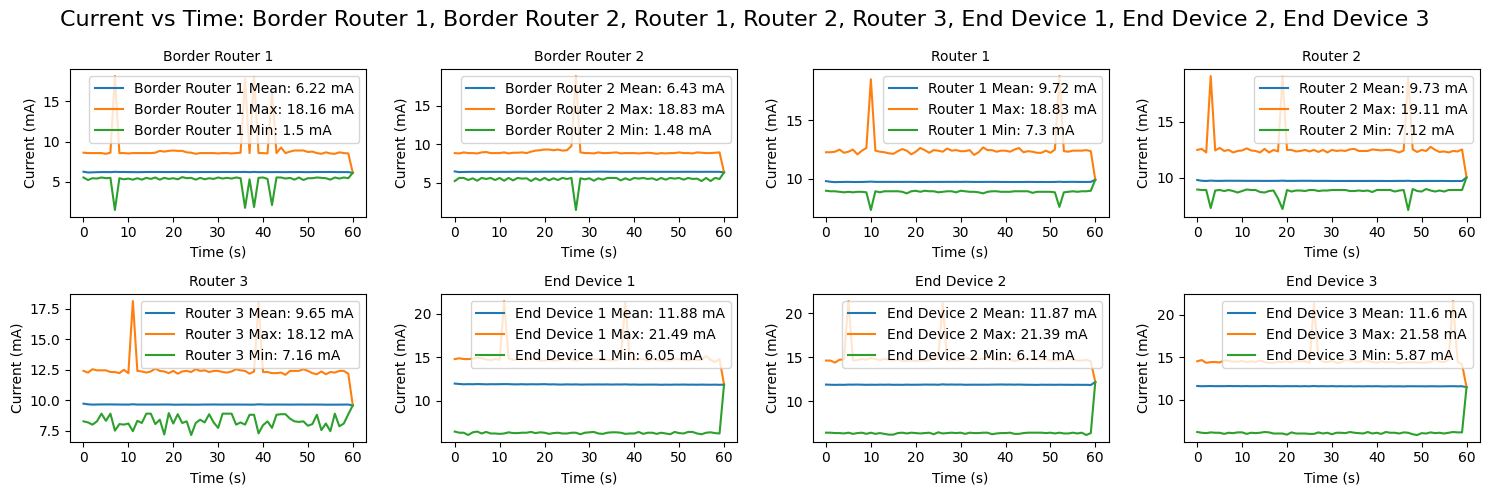
\includegraphics[width=1\textwidth]{images/research_results/current_consumption_analysis/maximum/lab/no_sensor/overview.png}
    \caption{Current consumption overview from individual devices in Lab location, No Sensor mode.}
    \label{fig:current_consumption_lab_no_sensor_overview}
\end{figure}

\begin{longtblr}[
  caption = {Current consumption overview from individual devices in Lab location, No Sensor mode.},
  label = {tab:current_consumption_lab_no_sensor_overview},
  ]{
  colspec = {X[l] X[l] X[l] X[l] X[l] X[l] X[l]},
  hlines, vlines,
  rowhead = 1, % Repeat the header row on every page
  row{1} = {font=\bfseries},
}
  Device & Input xpower $(dBm)$ & Total Ping & Mean $(mA)$ & Max $(mA)$ & Min $(mA)$ \\
  Border Router 1 & \SetCell[r=8]{c} 8 & \SetCell[r=8]{c} 0 & 6.22 & 18.16 & 1.5 \\
  Border Router 2 &  &  & 6.43 & 18.83 & 1.48 \\
  Router 1 &  &  & 9.72 & 18.83 & 7.3 \\
  Router 2 &  &  & 9.73 & 19.11 & 7.12 \\
  Router 3 &  &  & 9.65 & 18.12 & 7.16 \\
  End device 1 &  &  & 11.88 & 21.49 & 6.05 \\
  End device 2 &  &  & 11.87 & 21.39 & 6.14 \\
  End device 3 &  &  & 11.6 & 21.58 & 5.87 \\
\end{longtblr}


\paragraph{Mode: Ping}
The following plot and table provide an overview of the current consumption across the entire network in Ping mode, where devices actively send pings to their radios at regular intervals. This increased communication leads to higher power consumption.

\begin{figure}[H]
  \centering
  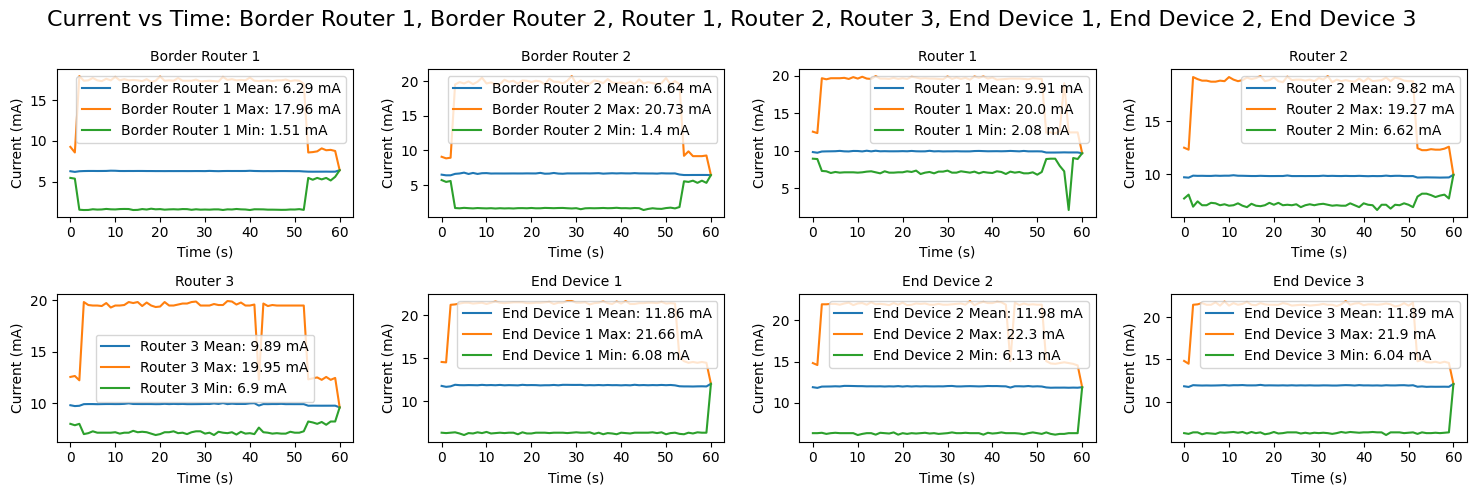
\includegraphics[width=1\textwidth]{images/research_results/current_consumption_analysis/maximum/lab/ping/overview.png}
    \caption{Current consumption overview from individual devices in Lab location, Ping mode.}
    \label{fig:current_consumption_lab_ping_overview}
\end{figure}

\begin{longtblr}[
  caption = {Current consumption overview from individual devices in Lab location, Ping mode.},
  label = {tab:current_consumption_lab_ping_overview},
  ]{
  colspec = {X[l] X[l] X[l] X[l] X[l] X[l] X[l]},
  hlines, vlines,
  rowhead = 1, % Repeat the header row on every page
  row{1} = {font=\bfseries},
}
  Device & Input txpower $(dBm)$ & Total Ping & Mean $(mA)$ & Max $(mA)$ & Min $(mA)$ \\
  Border Router 1 & \SetCell[r=8]{c} 8 & \SetCell[r=8]{c} 50 & 6.29 & 17.96 & 1.51 \\
  Border Router 2 &  &  & 6.64 & 20.73 & 1.4 \\
  Router 1 &  &  & 9.91 & 20.0 & 2.08 \\
  Router 2 &  &  & 9.82 & 19.27 & 6.62 \\
  Router 3 &  &  & 9.89 & 19.95 & 6.9 \\
  End device 1 &  &  & 11.86 & 21.66 & 6.08 \\
  End device 2 &  &  & 11.98 & 22.3 & 6.13 \\
  End device 3 &  &  & 11.89 & 21.9 & 6.04 \\
\end{longtblr}

\paragraph{Mode: Ultra-Wide Band}
In addition to No Sensor and Ping modes, another mode involves receiving data from an Ultra-Wide Band (UWB) network formed with ESP32 UWB devices shown in the research design section. The plot and table below showcase the current consumption in UWB mode, where devices utilize wide bandwidth for communication, resulting in higher power consumption across the network.

\begin{figure}[H]
  \centering
  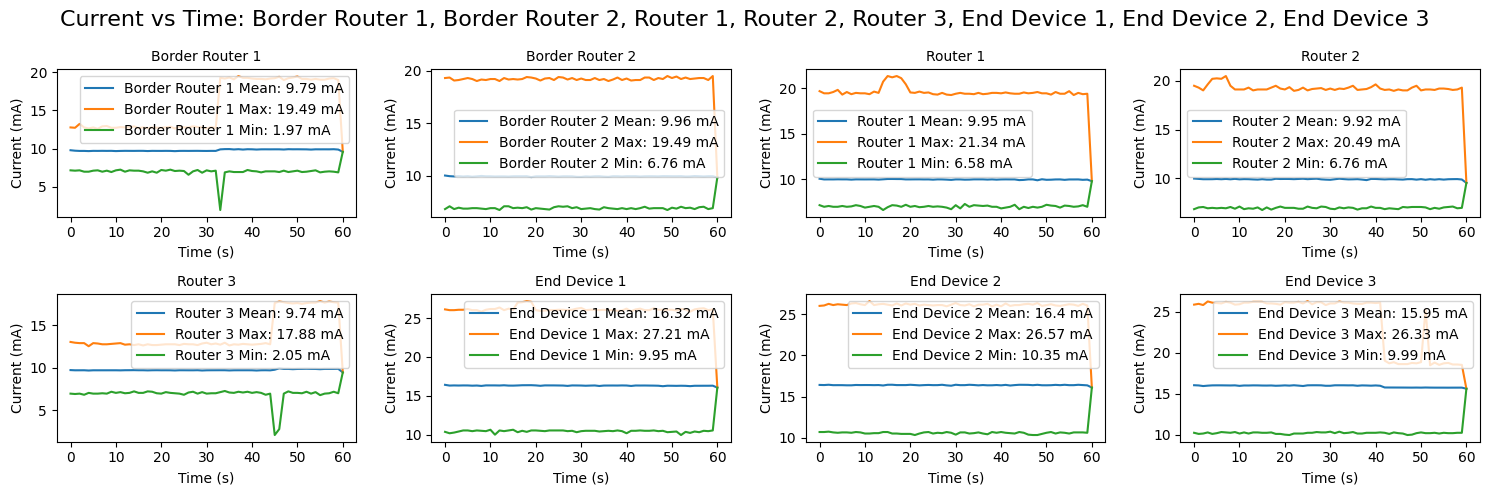
\includegraphics[width=1\textwidth]{images/research_results/current_consumption_analysis/maximum/lab/uwb/overview.png}
    \caption{Current consumption overview from individual devices in Lab location, UWB mode.}
    \label{fig:current_consumption_lab_uwb_overview}
\end{figure}

\begin{longtblr}[
  caption = {Current consumption overview from individual devices in Lab location, UWB mode.},
  label = {tab:current_consumption_lab_uwb_overview},
  ]{
  colspec = {X[l] X[l] X[l] X[l] X[l] X[l] X[l]},
  hlines, vlines,
  rowhead = 1, % Repeat the header row on every page
  row{1} = {font=\bfseries},
}
  Device & Input txpower $(dBm)$ & Total Ping & Mean $(mA)$ & Max $(mA)$ & Min $(mA)$ \\
  Border Router 1 & \SetCell[r=8]{c} 8 & \SetCell[r=8]{c} 5 per second (average) & 9.79 & 19.49 & 1.97 \\
  Border Router 2 &  &  & 9.96 & 19.49 & 6.76 \\
  Router 1 &  &  & 9.95 & 21.34 & 6.58 \\
  Router 2 &  &  & 9.92 & 20.49 & 6.76 \\
  Router 3 &  &  & 9.74 & 17.88 & 2.05 \\
  End device 1 &  &  & 16.32 & 27.21 & 9.95 \\
  End device 2 &  &  & 16.4 & 26.57 & 10.35 \\
  End device 3 &  &  & 15.95 & 26.33 & 9.99 \\
\end{longtblr}

\paragraph{Comparison: No Sensor vs. Ping vs. UWB}
The following plots compare the current consumption of the network in No Sensor, Ping, and Ultra-Wide Band (UWB) modes, highlighting the differences in power usage among the various communication methods.

\begin{figure}[H]
  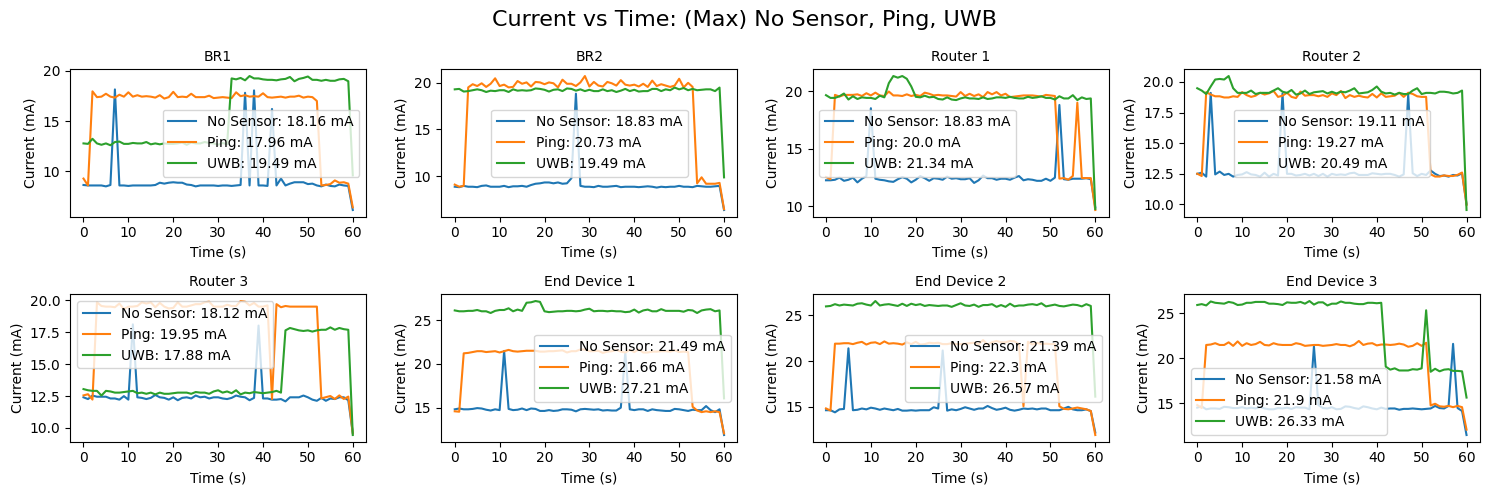
\includegraphics[width=1\textwidth]{images/research_results/current_consumption_analysis/maximum/lab/max_comparison_no-sensor_vs_ping_vs_uwb.png}
  \caption{Mean Current Consumption Comparison in Lab location, No Sensor vs. Ping vs. UWB modes.}
  \label{fig:mean_comparison_no-sensor_vs_ping_vs_uwb_lab}
\end{figure}

\begin{figure}[H]
  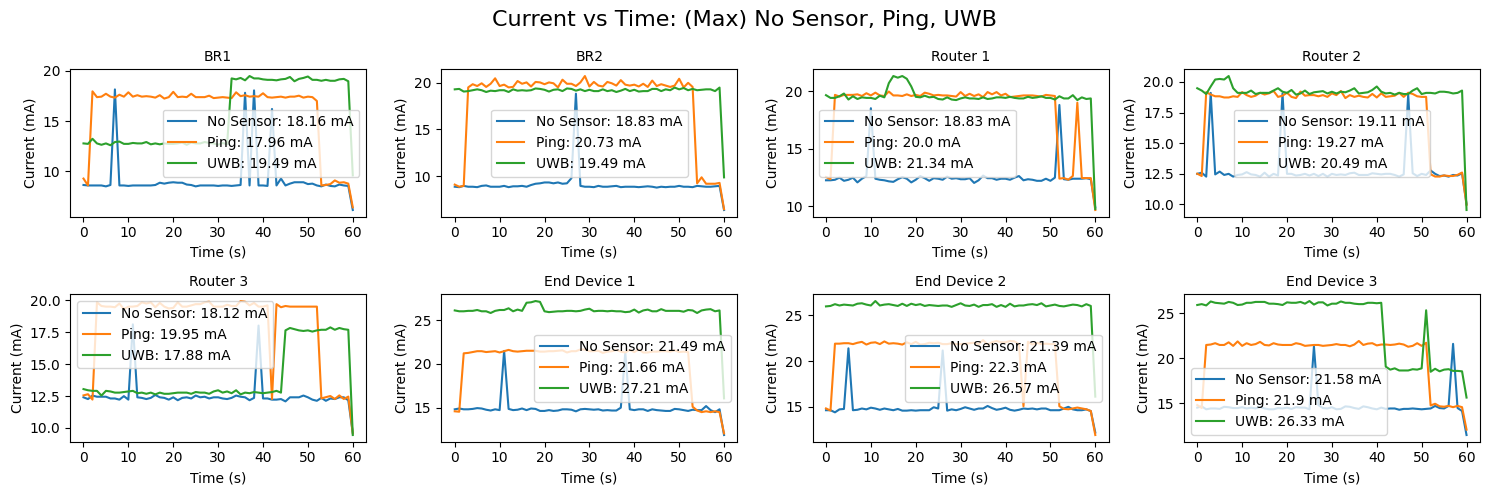
\includegraphics[width=1\textwidth]{images/research_results/current_consumption_analysis/maximum/lab/max_comparison_no-sensor_vs_ping_vs_uwb.png}
  \caption{Maximum Current Consumption Comparison in Lab location, No Sensor vs. Ping vs. UWB modes.}
  \label{fig:max_comparison_no-sensor_vs_ping_vs_uwb_lab}
\end{figure}

\begin{figure}[H]
  \centering
  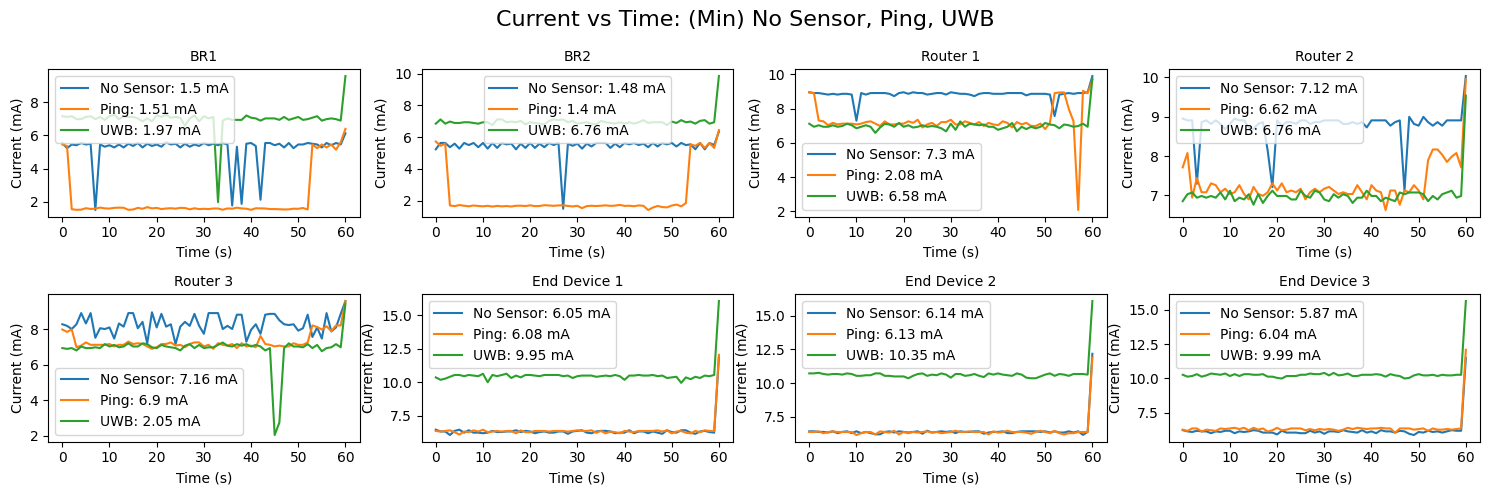
\includegraphics[width=1\textwidth]{images/research_results/current_consumption_analysis/maximum/lab/min_comparison_no-sensor_vs_ping_vs_uwb.png}
  \caption{Minimum Current Consumption Comparison in Lab location, No Sensor vs. Ping vs. UWB modes.}
  \label{fig:min_comparison_no-sensor_vs_ping_vs_uwb_lab}
\end{figure}

All the Figures above comprehensively compare current consumption measurements across devices operating in three modes: No Sensor, Ping, and UWB. Each device was set to a maximum transmission power of 8 $dBm$. In the No Sensor and Ping modes, 50 pings were sent over a 60-second duration, while in the UWB mode, 5 pings were sent each second for the entire 60-second period, resulting in a significantly higher number of pings.

As expected, due to the lack of radioactivity, the No Sensor mode demonstrates the lowest mean current consumption for all device types. Border Routers range from 6.22 to 6.43 $mA$, Routers from 9.65 to 9.73 $mA$, and End devices from 11.6 to 11.88 $mA$. The Ping mode shows a slight increase in mean current consumption for all devices, attributed to the radio usage for transmitting pings. In contrast, the UWB mode reveals a more pronounced change, particularly for End devices, which experience a significant jump to between 15.95 and 16.4 $mA$ due to the increased radioactivity and higher frequency of pings.

The maximum and minimum current consumption values also vary among the different modes. The higher number of pings in the UWB mode contributes to the increased current consumption, especially for End devices. This observation highlights the impact of communication frequency and radioactivity on power requirements.

\subsubsection{Location: Home}
This section focuses on the home location, which features a more significant distance between devices than the lab setting. The accompanying plot and table illustrate the impact of this increased distance on the network's current consumption.

\paragraph{Mode: No Sensor}
The following plot and table display the current consumption of devices in No Sensor mode at the home location, demonstrating the impact of reduced radio communication on power usage in this setting.

\begin{figure}[H]
  \centering
  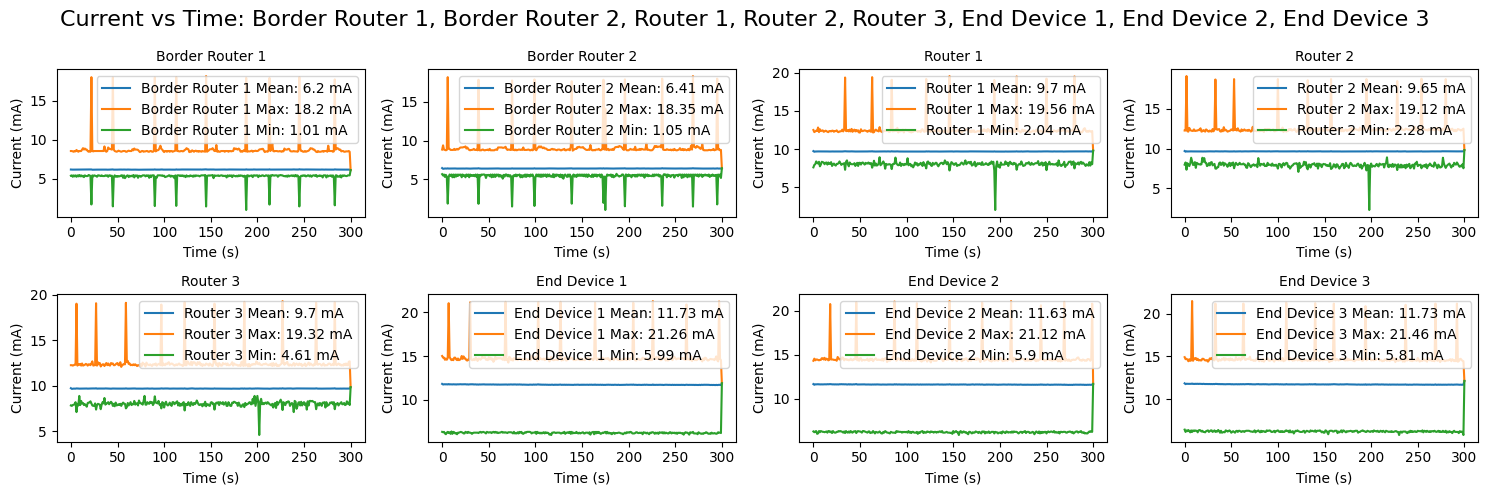
\includegraphics[width=1\textwidth]{images/research_results/current_consumption_analysis/maximum/home/no_sensor/overview.png}
    \caption{Current consumption overview from individual devices in Home location, No Sensor mode.}
    \label{fig:current_consumption_home_no-sensor_overview}
\end{figure}

\begin{longtblr}[
  caption = {Current consumption overview from individual devices in Home location, No Sensor mode.},
  label = {tab:current_consumption_home_no-sensor_overview},
  ]{
  colspec = {X[l] X[l] X[l] X[l] X[l] X[l] X[l]},
  hlines, vlines,
  rowhead = 1, % Repeat the header row on every page
  row{1} = {font=\bfseries},
}
  Device & Input txpower $(dBm)$ & Total Ping & Mean $(mA)$ & Max $(mA)$ & Min $(mA)$ \\
  Border Router 1 & \SetCell[r=8]{c} 8\ dBm & \SetCell[r=8]{c} 0 & 6.62 & 18.2 & 1.01 \\
  Border Router 2 &  &  & 6.41 & 18.35 & 1.05 \\
  Router 1 &  &  & 9.7 & 19.56 & 2.04 \\
  Router 2 &  &  & 9.65 & 19.12 & 2.28 \\
  Router 3 &  &  & 9.7 & 19.32 & 4.61 \\
  End device 1 &  &  & 11.73 & 21.26 & 5.99 \\
  End device 2 &  &  & 11.63 & 21.12 & 5.9 \\
  End device 3 &  &  & 11.73 & 21.46 & 5.81 \\
\end{longtblr}

\paragraph{Comparison: Lab No Sensor vs Home No Sensor}
In this section, a comparison is made between two different locations, considering the first 60 seconds of data from the Home location out of 300 seconds.

\begin{figure}[H]
  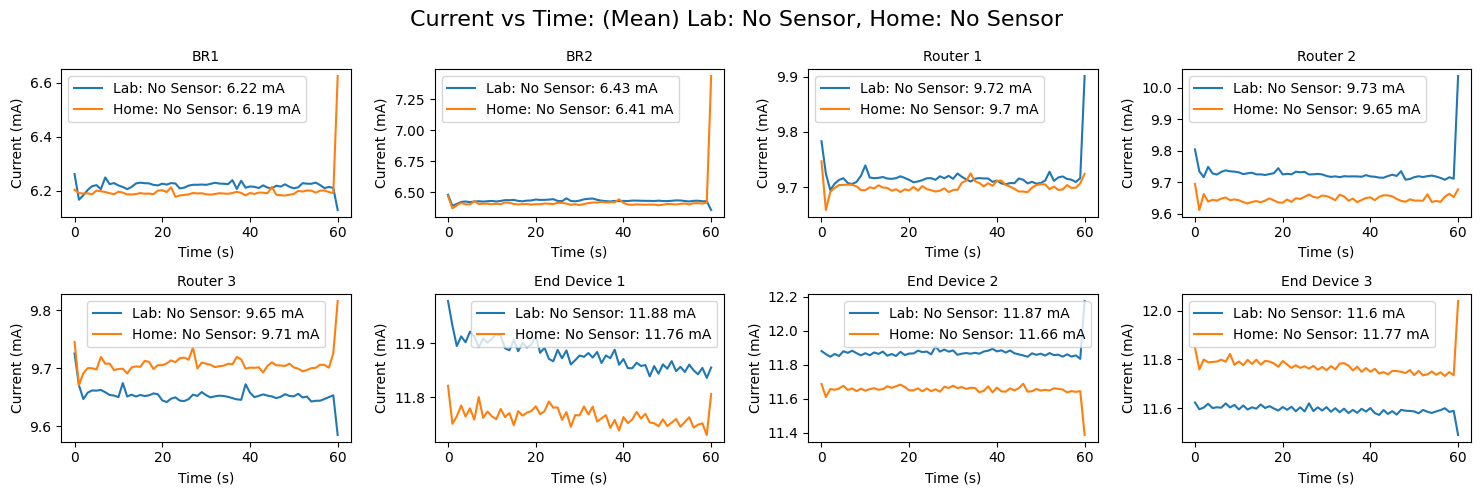
\includegraphics[width=1\textwidth]{images/research_results/current_consumption_analysis/maximum/home/no_sensor/comparison/lab_no-sensor_vs_home_no-sensor/mean_comparison_lab_vs_home.png}
  \caption{Mean Current Consumption Comparison in Home location, No Sensor mode vs. Lab location, No Sensor mode.}
  \label{fig:mean_comparison_lab_vs_home_no-sensor}
\end{figure}

\begin{figure}[H]
  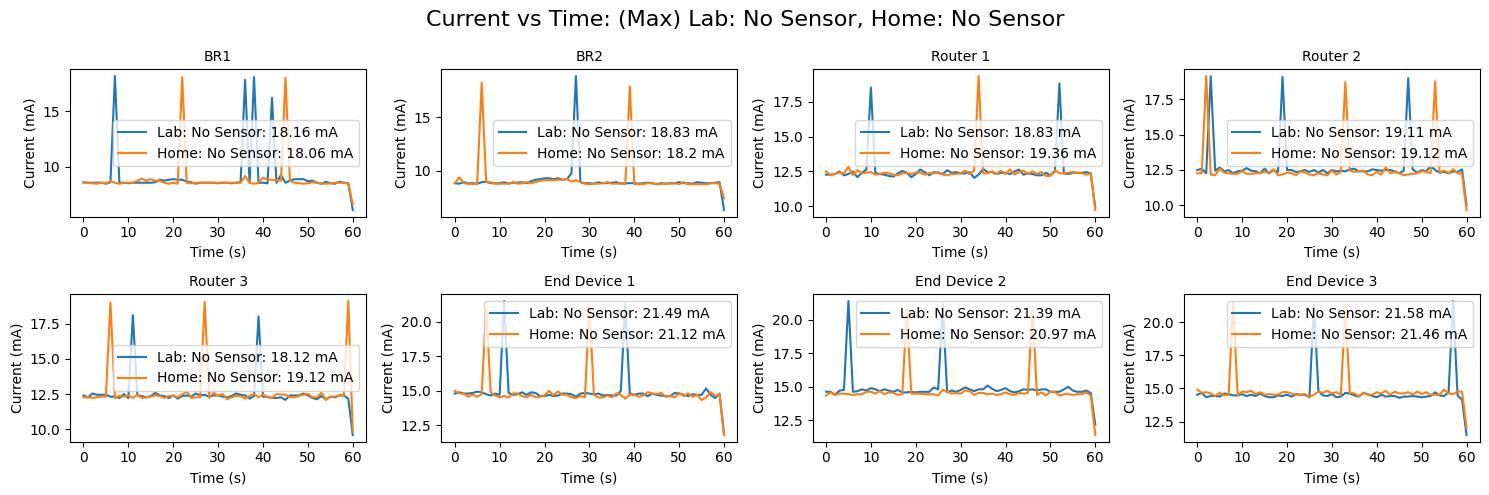
\includegraphics[width=1\textwidth]{images/research_results/current_consumption_analysis/maximum/home/no_sensor/comparison/lab_no-sensor_vs_home_no-sensor/max_comparison_lab_vs_home.png}
  \caption{Maximum Current Consumption Comparison in Home location, No Sensor mode vs. Lab location, No Sensor mode.}
  \label{fig:max_comparison_lab_vs_home_no-sensor}
\end{figure}

\begin{figure}[H]
  \centering
    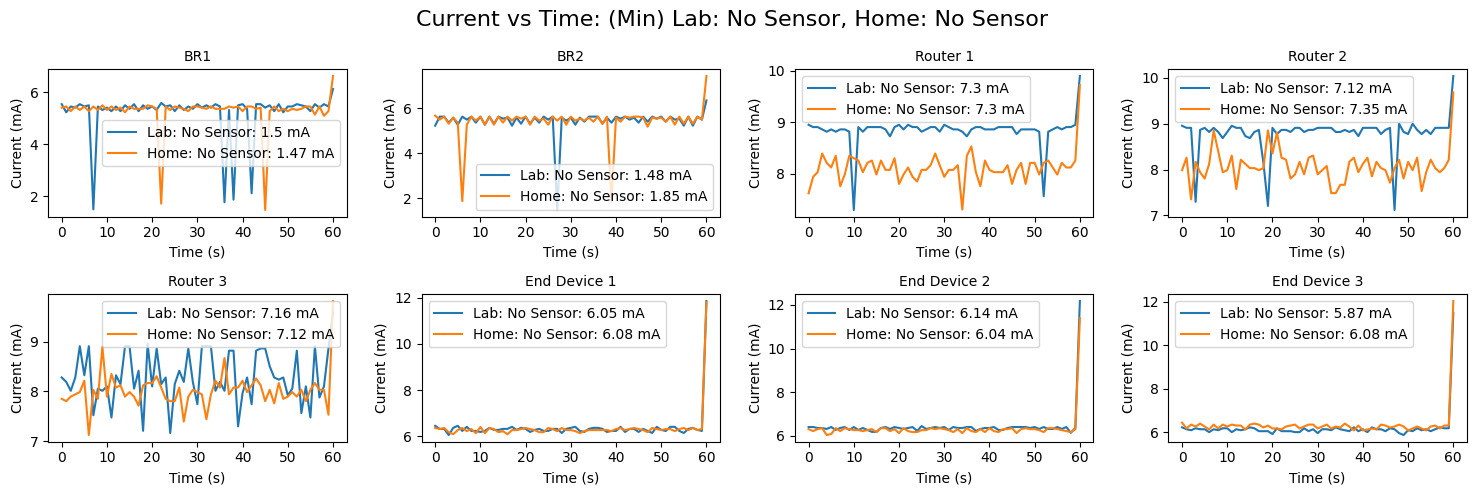
\includegraphics[width=1\textwidth]{images/research_results/current_consumption_analysis/maximum/home/no_sensor/comparison/lab_no-sensor_vs_home_no-sensor/min_comparison_lab_vs_home.png}
    \caption{Minimum Current Consumption Comparison in Home location, No Sensor mode vs. Lab location, No Sensor mode.}
    \label{fig:min_comparison_lab_vs_home_no-sensor}
\end{figure}

The accompanying graphs compare the No Sensor modes in two locations for current consumption in terms of mean, maximum, and minimum values. The results reveal that the power consumption is generally similar between Lab and Home environments, with slight variations among the devices. Border Routers 1 and 2 show marginally higher mean values in the Home environment, while Routers 1, 2, and 3 and End Devices 1, 2, and 3 exhibit minimal differences between the two domains.

\paragraph{Mode: Ping}
The following plot and table display the current consumption data for devices operating in Ping mode within the Home environment, providing insights into the power usage while actively sending pings.

\begin{figure}[H]
  \centering
  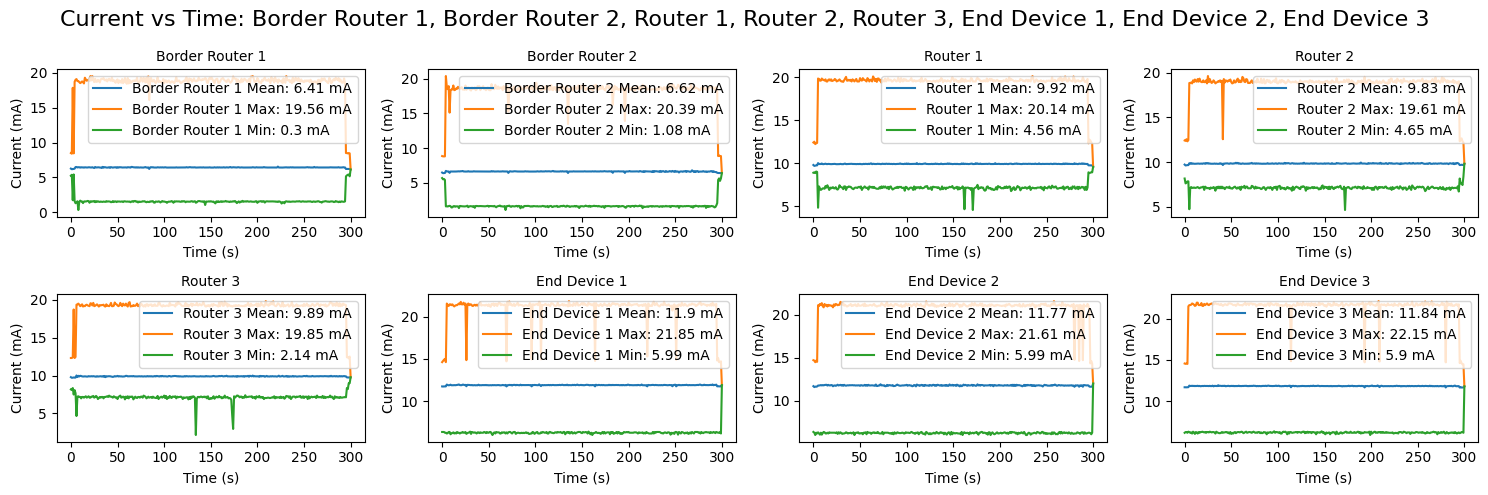
\includegraphics[width=1\textwidth]{images/research_results/current_consumption_analysis/maximum/home/ping/overview.png}
    \caption{Current consumption overview from individual devices in Home location, Ping mode.}
    \label{fig:current_consumption_home_ping_overview}
\end{figure}

\begin{longtblr}[
  caption = {Current consumption overview from individual devices in Lab location.},
  label = {tab:current_consumption_lab_overview},
  ]{
  colspec = {X[l] X[l] X[l] X[l] X[l] X[l] X[l]},
  hlines, vlines,
  rowhead = 1, % Repeat the header row on every page
  row{1} = {font=\bfseries},
}
  Device & Input txpower $(dBm)$ & Total Ping & Mean $(mA)$ & Max $(mA)$ & Min $(mA)$ \\
  Border Router 1 & \SetCell[r=8]{c} 8 & \SetCell[r=8]{c} 290 & 6.41 & 19.56 & 0.3 \\
  Border Router 2 &  &  & 6.62 & 20.39 & 1.08 \\
  Router 1 &  &  & 9.92 & 20.14 & 4.56 \\
  Router 2 &  &  & 9.83 & 19.61 & 4.65 \\
  Router 3 &  &  & 9.89 & 19.85 & 2.14 \\
  End device 1 &  &  & 11.9 & 21.85 & 5.99 \\
  End device 2 &  &  & 11.77 & 21.61 & 5.99 \\
  End device 3 &  &  & 11.84 & 22.15 & 5.99 \\
\end{longtblr}

\paragraph{Comparison: Home No Sensor vs. Home Ping}
The following plots showcase a comparison between No Sensor and Ping modes in the Home environment, providing an overview of the differences in current consumption when devices operate passively without sending pings and when actively sending pings in the network.

\begin{figure}[H]
  \centering
  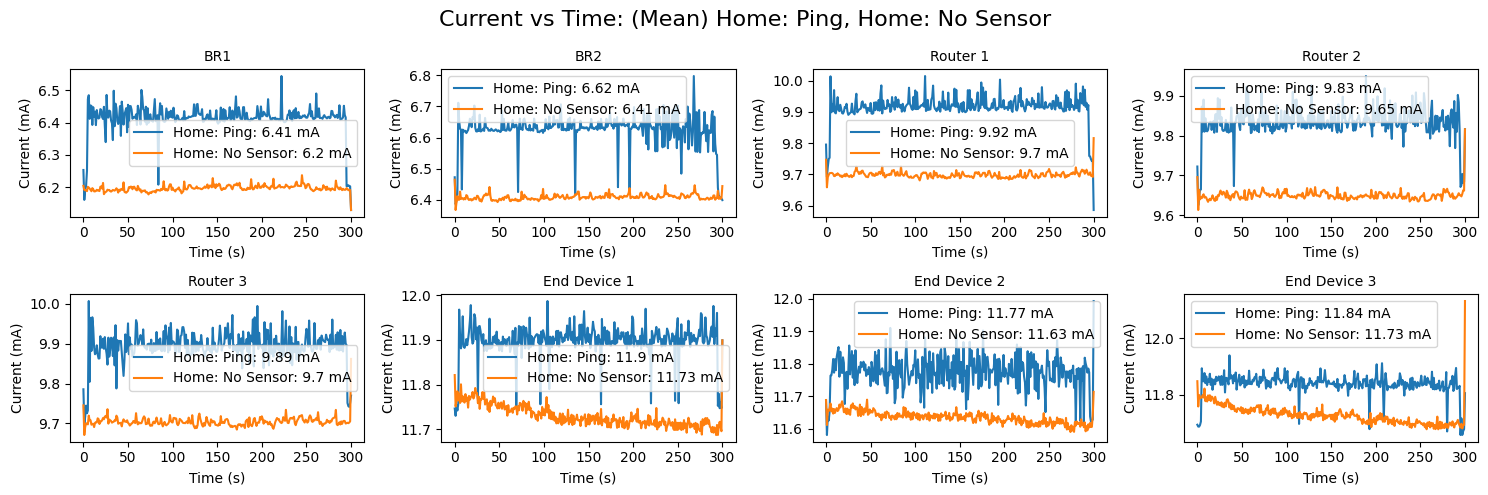
\includegraphics[width=1\textwidth]{images/research_results/current_consumption_analysis/maximum/home/ping/comparison/home_no-sensor_vs_home_ping/mean_comparison_home_no-sensor_vs_home_ping.png}
    \caption{Mean Current Consumption Comparison in Home location, No Sensor mode vs. Home location, Ping mode.}
    \label{fig:mean_comparison_home_no-sensor_vs_home_ping}
\end{figure}

\begin{figure}[H]
  \centering
  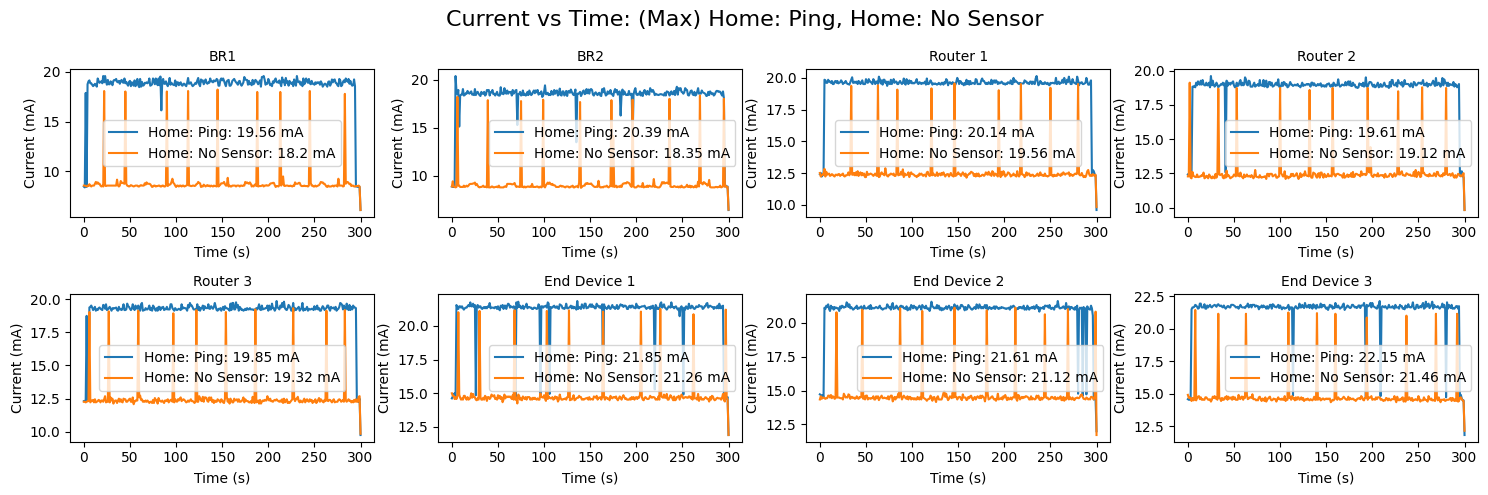
\includegraphics[width=1\textwidth]{images/research_results/current_consumption_analysis/maximum/home/ping/comparison/home_no-sensor_vs_home_ping/max_comparison_home_no-sensor_vs_home_ping.png}
    \caption{Maximum Current Consumption Comparison in Home location, No Sensor mode vs. Home location, Ping mode.}
    \label{fig:max_comparison_home_no-sensor_vs_home_ping}
\end{figure}

\begin{figure}[H]
  \centering
  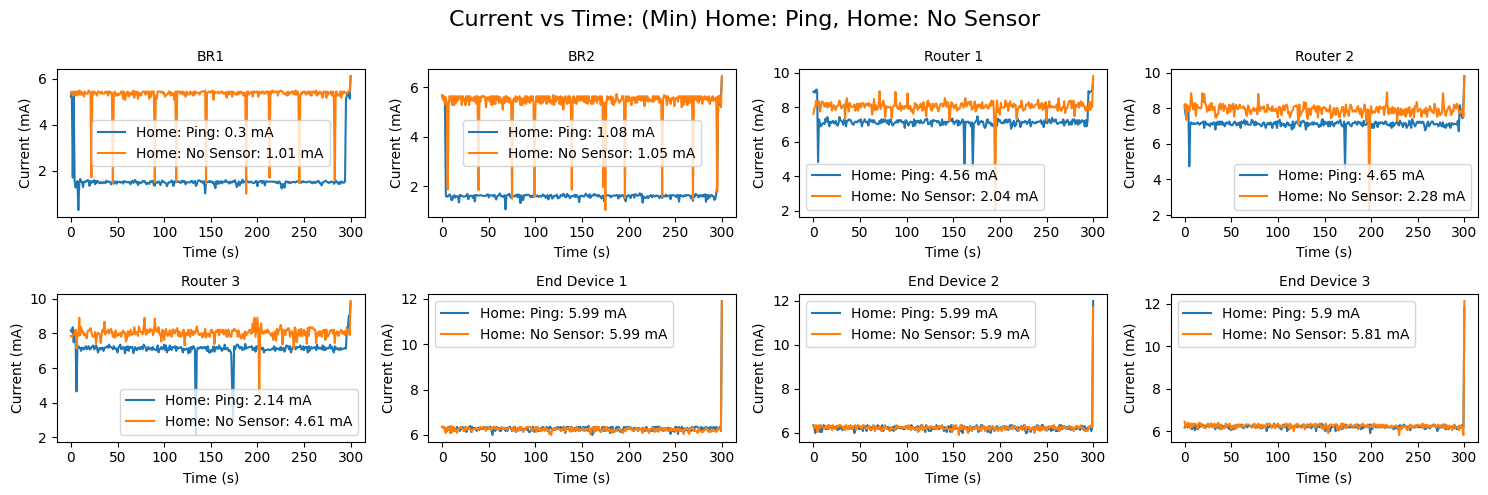
\includegraphics[width=1\textwidth]{images/research_results/current_consumption_analysis/maximum/home/ping/comparison/home_no-sensor_vs_home_ping/min_comparison_home_no-sensor_vs_home_ping.png}
    \caption{Minimum Current Consumption Comparison in Home location, No Sensor mode vs. Home location, Ping mode.}
    \label{fig:min_comparison_home_no-sensor_vs_home_ping}
\end{figure}

The comparison of the Home location's No Sensor and Ping modes highlights the differences in current consumption for each device in the network. The Ping mode generally has slightly higher mean current consumption for most devices, except for the border routers. The maximum and minimum current consumption values also vary between the two modes.

\paragraph{Comparison: Lab Ping vs. Home Ping}
The following plots compare different location's Ping modes, illustrating the differences in current consumption for other devices when actively sending pings in the network. Only the first 60 seconds of data from the Home Ping mode is considered to ensure a fair comparison.

\begin{figure}[H]
  \centering
  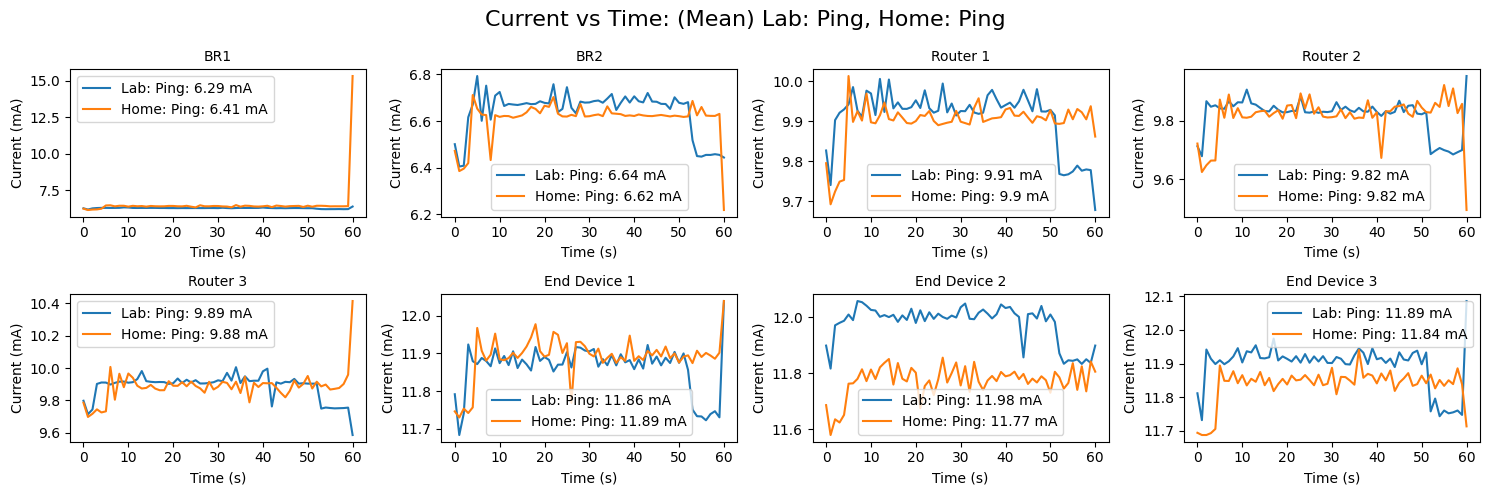
\includegraphics[width=1\textwidth]{images/research_results/current_consumption_analysis/maximum/home/ping/comparison/lab_ping_vs_home_ping/mean_comparison_lab_ping_vs_home_ping.png}
    \caption{Mean Current Consumption Comparison in Lab location, Ping mode vs. Home location, Ping mode.}
    \label{fig:mean_comparison_lab_ping_vs_home_ping}
\end{figure}

\begin{figure}[H]
  \centering
  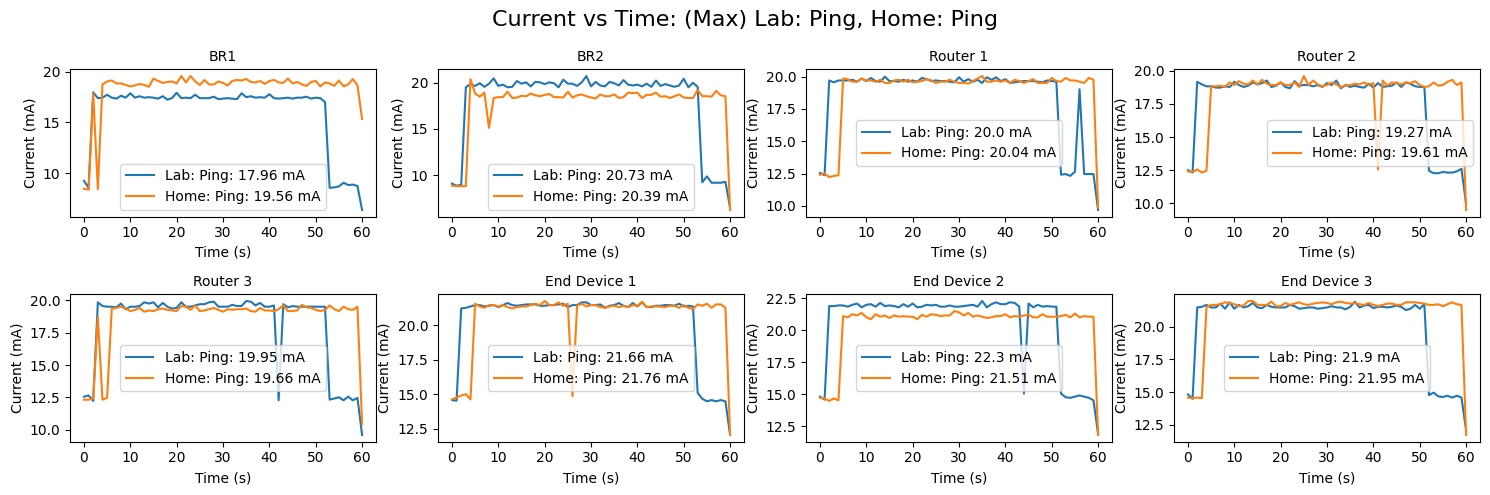
\includegraphics[width=1\textwidth]{images/research_results/current_consumption_analysis/maximum/home/ping/comparison/lab_ping_vs_home_ping/max_comparison_lab_ping_vs_home_ping.png}
    \caption{Maximum Current Consumption Comparison in Lab location, Ping mode vs. Home location, Ping mode.}
    \label{fig:max_comparison_lab_ping_vs_home_ping}
\end{figure}

\begin{figure}[H]
  \centering
  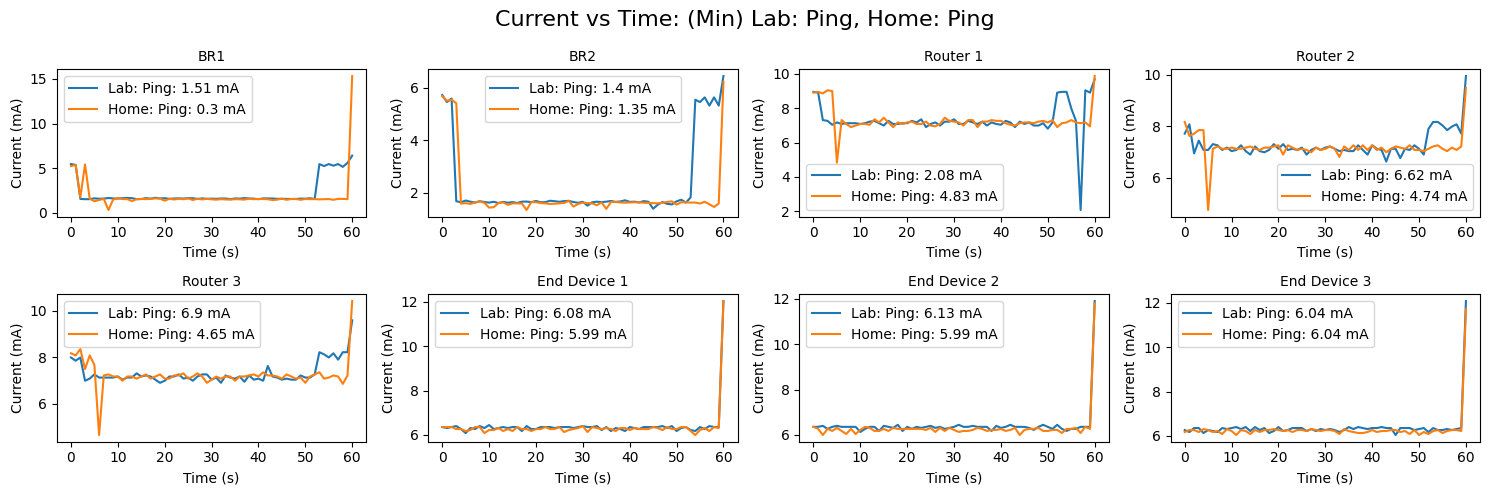
\includegraphics[width=1\textwidth]{images/research_results/current_consumption_analysis/maximum/home/ping/comparison/lab_ping_vs_home_ping/min_comparison_lab_ping_vs_home_ping.png}
    \caption{Minimum Current Consumption Comparison in Lab location, Ping mode vs. Home location, Ping mode.}
    \label{fig:min_comparison_lab_ping_vs_home_ping}
\end{figure}

The graphs compare power consumption between Lab and Home locations in Ping mode. The Lab location, being a smaller room, has lower distances between devices, resulting in a more efficient power consumption profile. On the other hand, the Home location has more considerable distances between devices, contributing to slightly higher current consumption in mean values for some devices. Maximum and minimum values also display minor variations between the Lab and Home environments, underscoring the impact of environmental factors and distances on power consumption.


\subsection{Optimized Current Consumption}
In this section, we explore the effects of applying Monte Carlo (MC) and Genetic Algorithm (GA) techniques to optimize transmission power for each device. This approach aims to minimize power consumption while maintaining reliable communication across the network, showcasing the benefits of implementing such optimization algorithms.

\subsubsection{Location: Lab}
Data and power consumption patterns are explored in this location when MC and GA algorithms are applied for transmission power optimization. This examination highlights the potential for improved power management within a confined space, emphasizing the importance of energy-efficient communication in such environments.

\paragraph{Mode: No Sensor}
This analysis focuses on idle device mode when devices aren’t actively sending pings. By applying MC and GA algorithms for transmission power optimization, the goal is to evaluate the impact of these methods on reducing power consumption.

\subparagraph{Monte Carlo Method}
The following plot and table showcase the Monte Carlo Method (MCM) optimized mode, which aims to meet mathematical constraints and deliver the correct network configuration with initial transmission power values.

\begin{figure}[H]
  \centering
  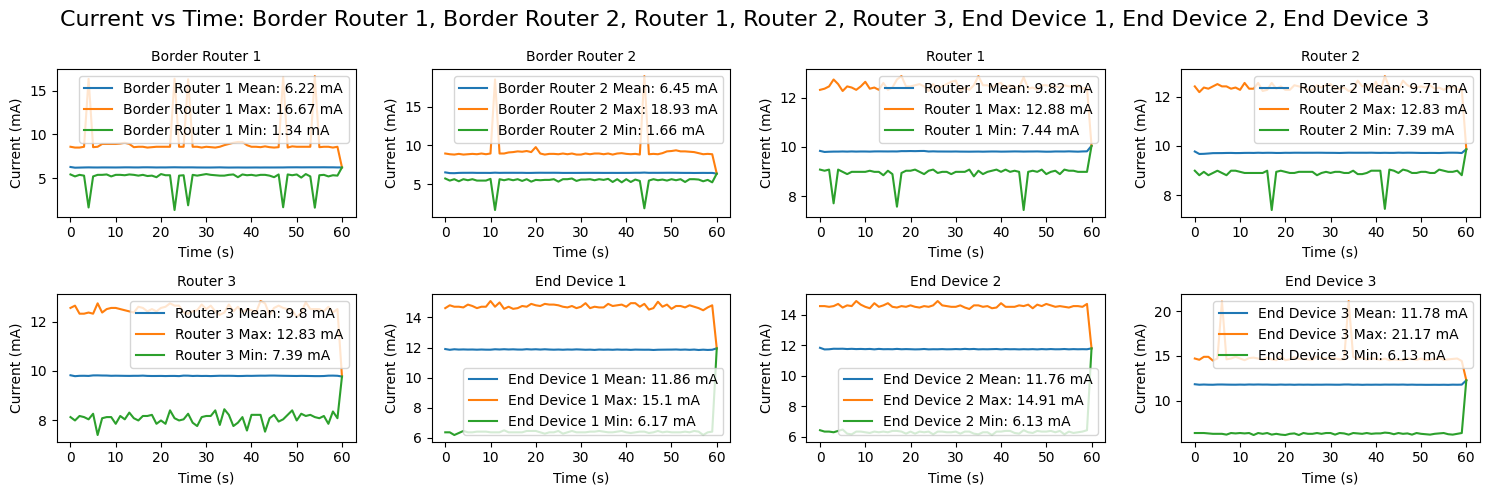
\includegraphics[width=1\textwidth]{images/research_results/current_consumption_analysis/optimized/lab/no_sensor/mc/overview.png}
    \caption{Overview of Current Consumption in Lab location, No Sensor mode, MCM optimized mode.}
    \label{fig:overview_lab_no-sensor_mc}
\end{figure}

\begin{longtblr}[
  caption = {Current Consumption in Lab location, No Sensor mode, MCM optimized mode.},
  label = {tab:lab_no-sensor_mc_overview},
  ]{
  colspec = {X[l] X[l] X[l] X[l] X[l] X[l] X[l]},
  hlines, vlines,
  rowhead = 1, % Repeat the header row on every page
  row{1} = {font=\bfseries},
}
  Device & Input txpower $(dBm)$ & Total Ping & Mean $(mA)$ & Max $(mA)$ & Min $(mA)$ \\
  Border Router 1 & -8 & \SetCell[r=8]{c} 0 & 6.22 & 16.67 & 1.34 \\
  Border Router 2 & 8 &  & 6.45 & 18.93 & 1.66 \\
  Router 1 & -16 &  & 9.82 & 12.88 & 7.44 \\
  Router 2 & 0 &  & 9.71 & 12.83 & 7.39 \\
  Router 3 & 0 &  & 9.8 & 12.83 & 7.39 \\
  End device 1 & -8 &  & 11.86 & 15.1 & 6.17 \\
  End device 2 & -20 &  & 11.76 & 14.91 & 6.13 \\
  End device 3 & 8 &  & 11.78 & 21.17 & 6.13 \\
\end{longtblr}

\subparagraph{Comparison: Maximum Lab No Sensor vs Optimized Lab No Sensor MCM}
The following plots provide a comparison highlighting the differences in power consumption when applying optimization techniques to reduce energy usage in a lab setting without sensor data transmission.

\begin{figure}[H]
  \centering
  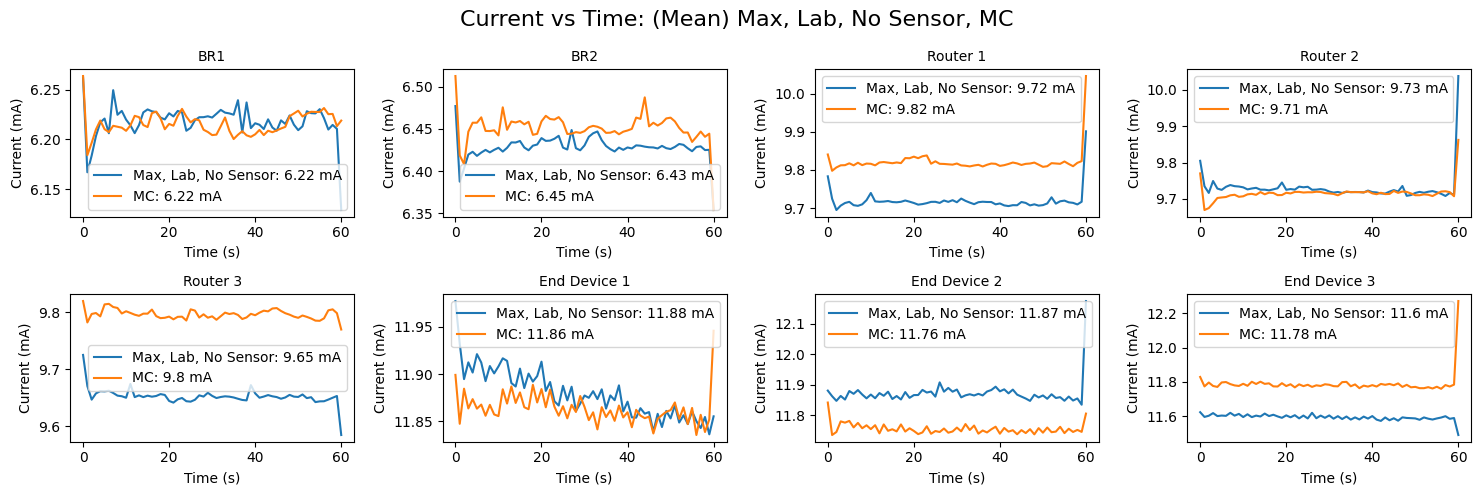
\includegraphics[width=1\textwidth]{images/research_results/current_consumption_analysis/optimized/lab/no_sensor/mc/comparison/mean_comparison_lab_no-sensor_vs_lab_no-sensor_mc.png}
    \caption{Mean Current Consumption Comparison in Lab location, No Sensor mode vs. Lab location, No Sensor mode, MCM optimized mode.}
    \label{fig:mean_comparison_lab_no-sensor_vs_lab_no-sensor_mc}
\end{figure}

\begin{figure}[H]
  \centering
  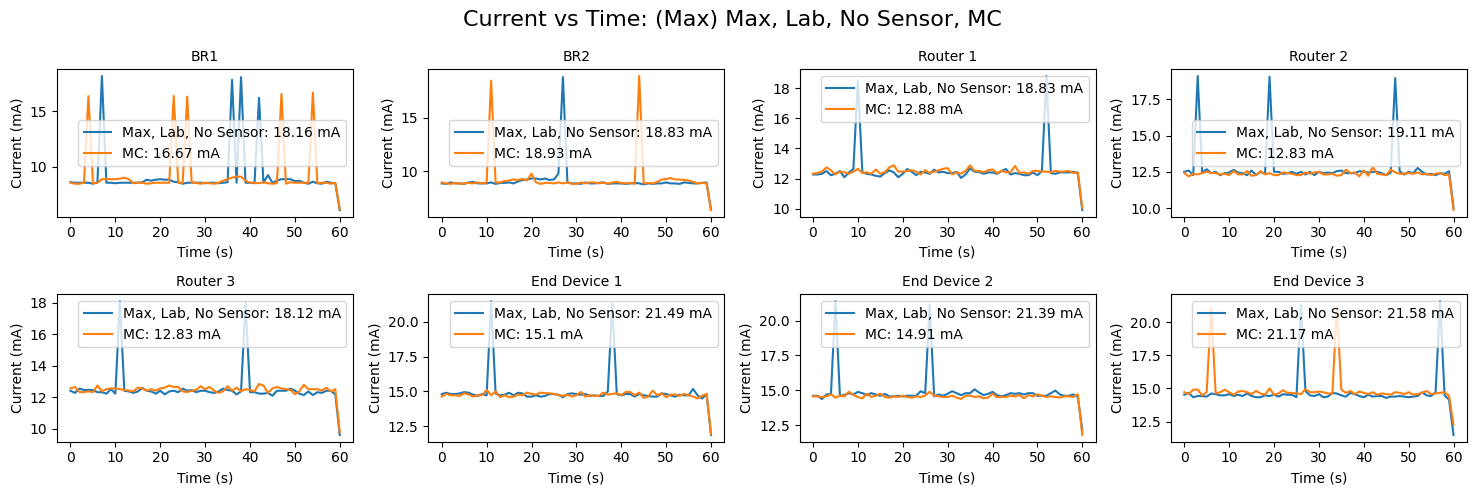
\includegraphics[width=1\textwidth]{images/research_results/current_consumption_analysis/optimized/lab/no_sensor/mc/comparison/max_comparison_lab_no-sensor_vs_lab_no-sensor_mc.png}
    \caption{Maximum Current Consumption Comparison in Lab location, No Sensor mode vs. Lab location, No Sensor mode, MCM optimized mode.}
    \label{fig:max_comparison_lab_no-sensor_vs_lab_no-sensor_mc}
\end{figure}

\begin{figure}[H]
  \centering
  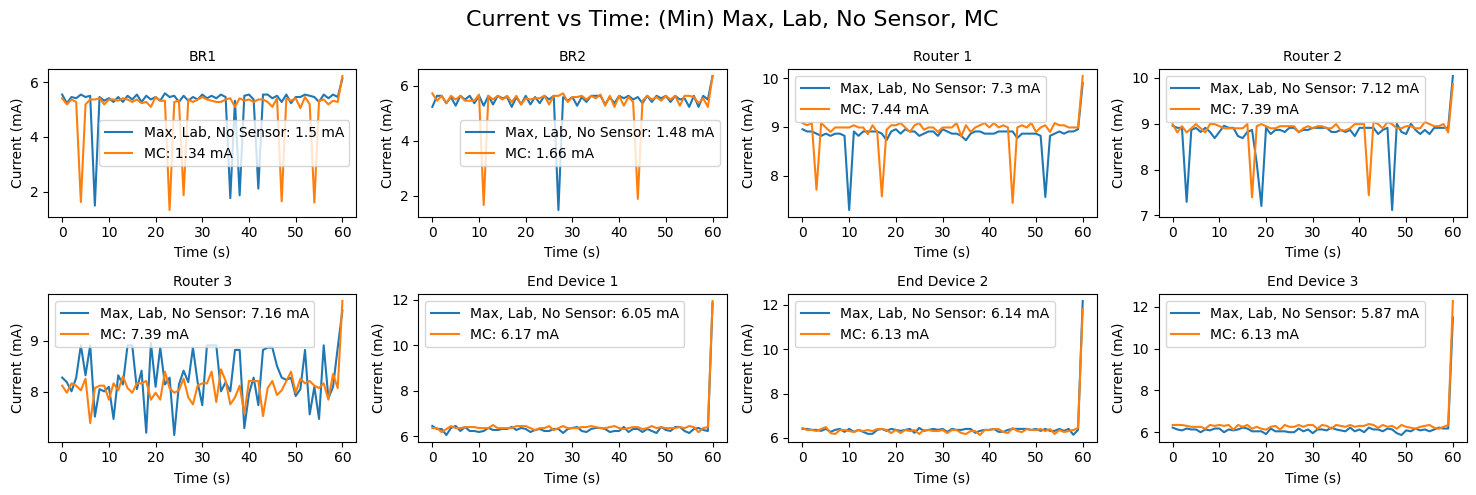
\includegraphics[width=1\textwidth]{images/research_results/current_consumption_analysis/optimized/lab/no_sensor/mc/comparison/min_comparison_lab_no-sensor_vs_lab_no-sensor_mc.png}
    \caption{Minimum Current Consumption Comparison in Lab location, No Sensor mode vs. Lab location, No Sensor mode, MCM optimized mode.}
    \label{fig:min_comparison_lab_no-sensor_vs_lab_no-sensor_mc}
\end{figure}

The comparison graphs show the Optimized mode improved current consumption, particularly for End devices and Routers with reduced transmission power. For instance, Router 1 has a maximum current consumption of 12.88 $mA$ in the optimized mode compared to 18.83 $mA$ in the maximum mode. Similarly, End device 2 shows a maximum current consumption of 14.91 $mA$ in the optimized mode compared to 21.39 $mA$ in the maximum mode.

\subparagraph{Genetic Algorithm}
The following plot and table showcase the power consumption results utilizing Genetic Algorithm (GA) that aims to reduce transmission power by satisfying mathematical constraints.

\begin{figure}[H]
  \centering
  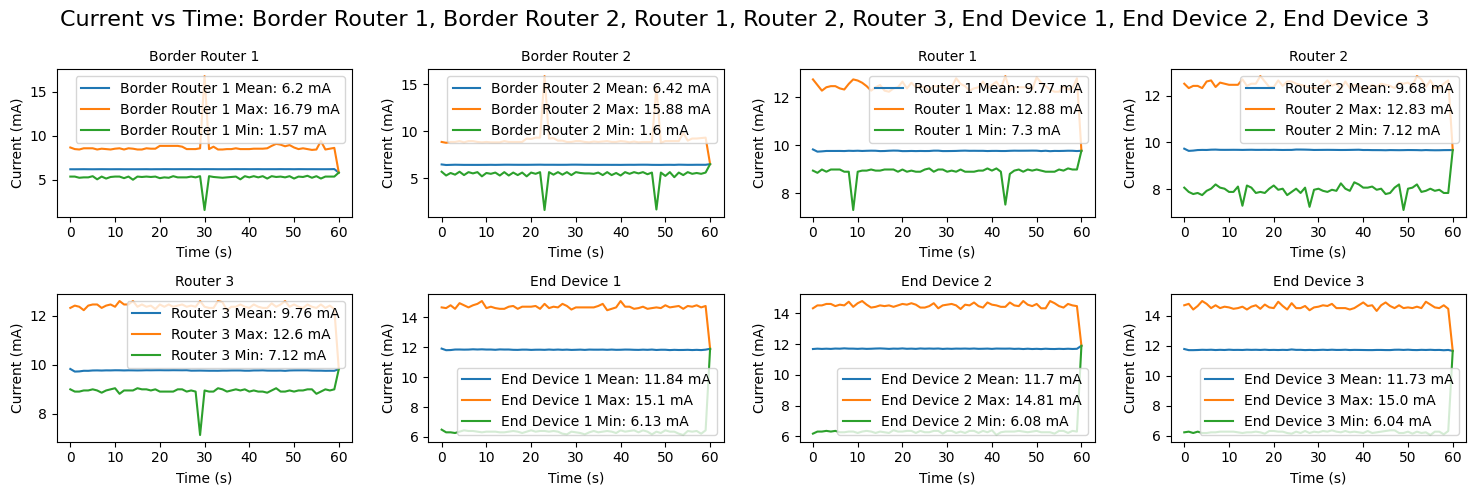
\includegraphics[width=1\textwidth]{images/research_results/current_consumption_analysis/optimized/lab/no_sensor/ga/overview.png}
    \caption{Overview of Current Consumption in Lab location, No Sensor mode, GA optimized mode.}
    \label{fig:overview_lab_no-sensor_ga}
\end{figure}

\begin{longtblr}[
  caption = {Current Consumption in Lab location, No Sensor mode, GA optimized mode.},
  label = {tab:lab_no-sensor_ga_overview},
  ]{
  colspec = {X[l] X[l] X[l] X[l] X[l] X[l] X[l]},
  hlines, vlines,
  rowhead = 1, % Repeat the header row on every page
  row{1} = {font=\bfseries},
}
  Device & Input txpower $(dBm)$ & Total Ping & Mean $(mA)$ & Max $(mA)$ & Min $(mA)$ \\
  Border Router 1 & \SetCell[r=8]{c} -20 & \SetCell[r=8]{c} 0 & 6.2 & 16.79 & 1.57 \\
  Border Router 2 &  &  & 6.42 & 15.88 & 1.6 \\
  Router 1 &  &  & 9.77 & 12.88 & 7.3 \\
  Router 2 &  &  & 9.68 & 12.83 & 7.12 \\
  Router 3 &  &  & 9.76 & 12.6 & 7.12 \\
  End device 1 &  &  & 11.84 & 15.1 & 6.13 \\
  End device 2 &  &  & 11.7 & 14.81 & 6.08 \\
  End device 3 &  &  & 11.73 & 15.0 & 6.04 \\
\end{longtblr}

\subparagraph{Comparison: Optimized Lab No Sensor MCM vs Optimized Lab GA}
This section compares MC and GA optimization approaches, showcasing their differences in power consumption through the following plots and table, highlighting the efficiency of each optimization technique.

\begin{figure}[H]
  \centering
  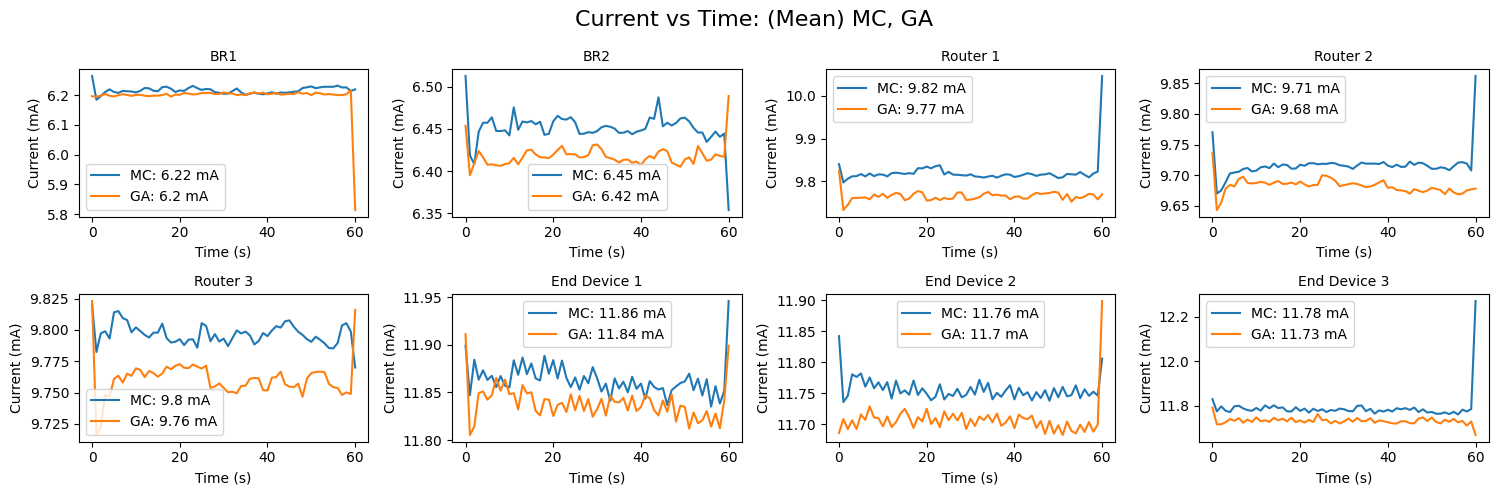
\includegraphics[width=1\textwidth]{images/research_results/current_consumption_analysis/optimized/lab/no_sensor/ga/comparison/mean_comparison_lab_no-sensor_mc_vs_lab_no-sensor_ga.png}
    \caption{Mean Current Consumption Comparison in Lab location, No Sensor mode, MCM optimized mode vs. Lab location, No Sensor mode, GA optimized mode.}
    \label{fig:mean_comparison_lab_no-sensor_mc_vs_lab_no-sensor_ga}
\end{figure}

\begin{figure}[H]
  \centering
  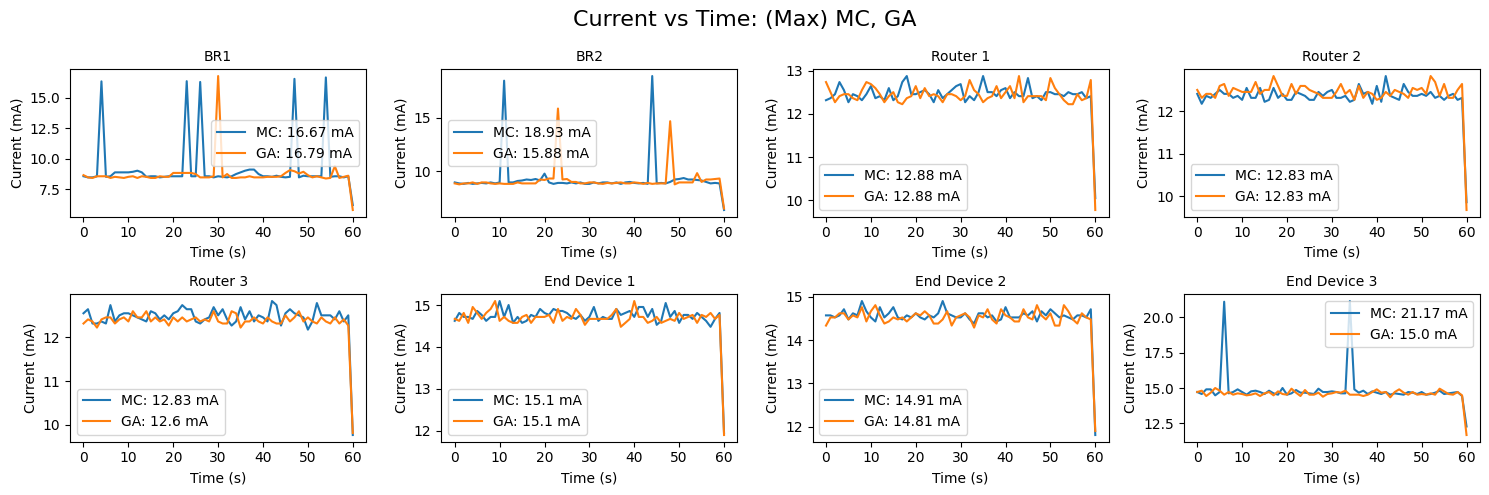
\includegraphics[width=1\textwidth]{images/research_results/current_consumption_analysis/optimized/lab/no_sensor/ga/comparison/max_comparison_lab_no-sensor_mc_vs_lab_no-sensor_ga.png}
    \caption{Maximum Current Consumption Comparison in Lab location, No Sensor mode, MCM optimized mode vs. Lab location, No Sensor mode, GA optimized mode.}
    \label{fig:max_comparison_lab_no-sensor_mc_vs_lab_no-sensor_ga}
\end{figure}

\begin{figure}[H]
  \centering
  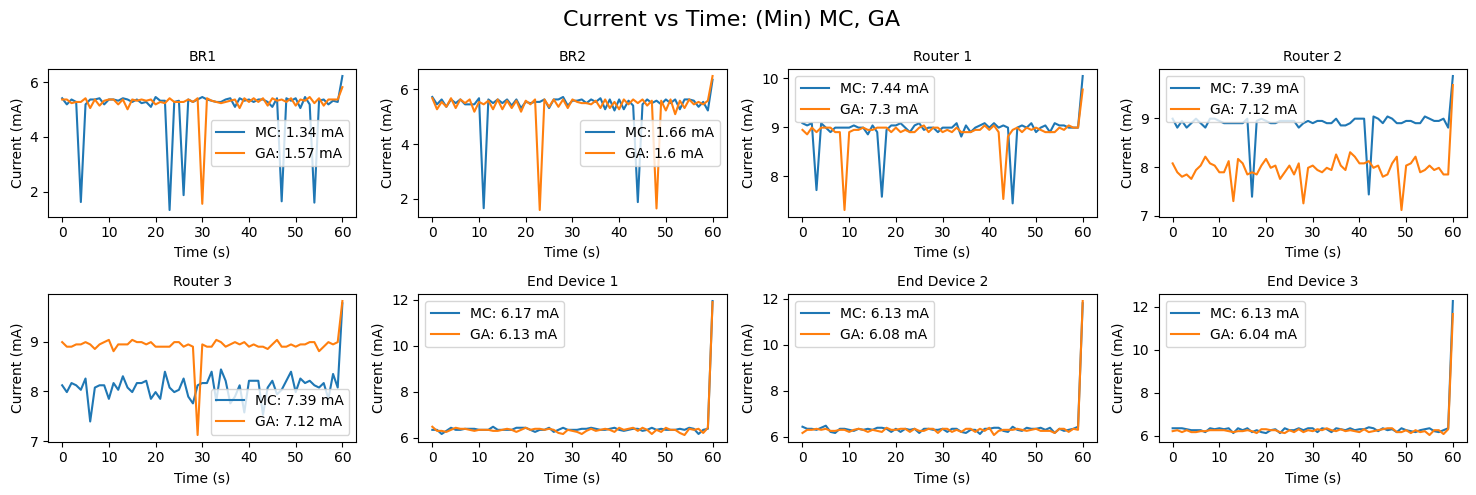
\includegraphics[width=1\textwidth]{images/research_results/current_consumption_analysis/optimized/lab/no_sensor/ga/comparison/min_comparison_lab_no-sensor_mc_vs_lab_no-sensor_ga.png}
    \caption{Minimum Current Consumption Comparison in Lab location, No Sensor mode, MCM optimized mode vs. Lab location, No Sensor mode, GA optimized mode.}
    \label{fig:min_comparison_lab_no-sensor_mc_vs_lab_no-sensor_ga}
\end{figure}

The graphs' comparison of MCM and GA modes highlights differences in current consumption across devices. Generally, GA mode shows the slightly lower mean, maximum, and minimum current consumption levels for most devices than MCM mode. With GA consistently used for all devices, the GA optimization approach may offer marginally better energy efficiency.

\subparagraph{Comparison: Maximum Lab No Sensor vs Optimized Lab No Sensor GA}
This section compares the Maximum mode with the Optimized mode, showcasing the total transmission power optimization achieved through the Genetic Algorithm, reducing current consumption while maintaining network performance.

\begin{figure}[H]
  \centering
  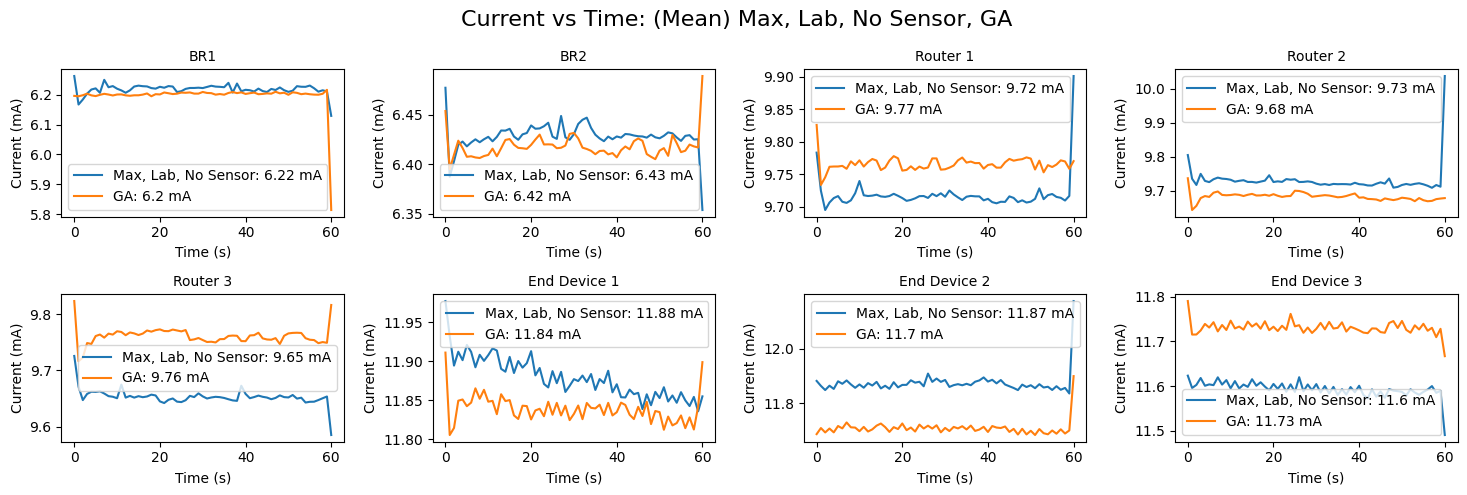
\includegraphics[width=1\textwidth]{images/research_results/current_consumption_analysis/optimized/lab/no_sensor/ga/comparison/mean_comparison_lab_no-sensor_vs_lab_no-sensor_ga.png}
    \caption{Mean Current Consumption Comparison in Lab location, No Sensor mode vs. Lab location, No Sensor mode, GA optimized mode.}
    \label{fig:mean_comparison_lab_no-sensor_vs_lab_no-sensor_ga}
\end{figure}

\begin{figure}[H]
  \centering
  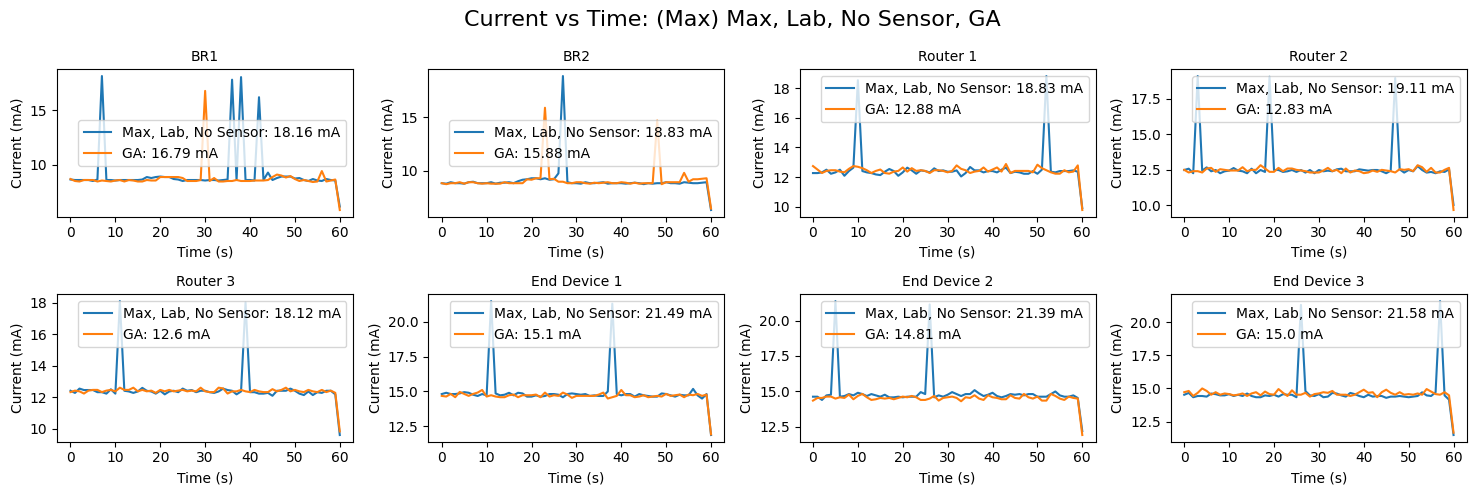
\includegraphics[width=1\textwidth]{images/research_results/current_consumption_analysis/optimized/lab/no_sensor/ga/comparison/max_comparison_lab_no-sensor_vs_lab_no-sensor_ga.png}
    \caption{Maximum Current Consumption Comparison in Lab location, No Sensor mode vs. Lab location, No Sensor mode, GA optimized mode.}
    \label{fig:max_comparison_lab_no-sensor_vs_lab_no-sensor_ga}
\end{figure}

\begin{figure}[H]
  \centering
  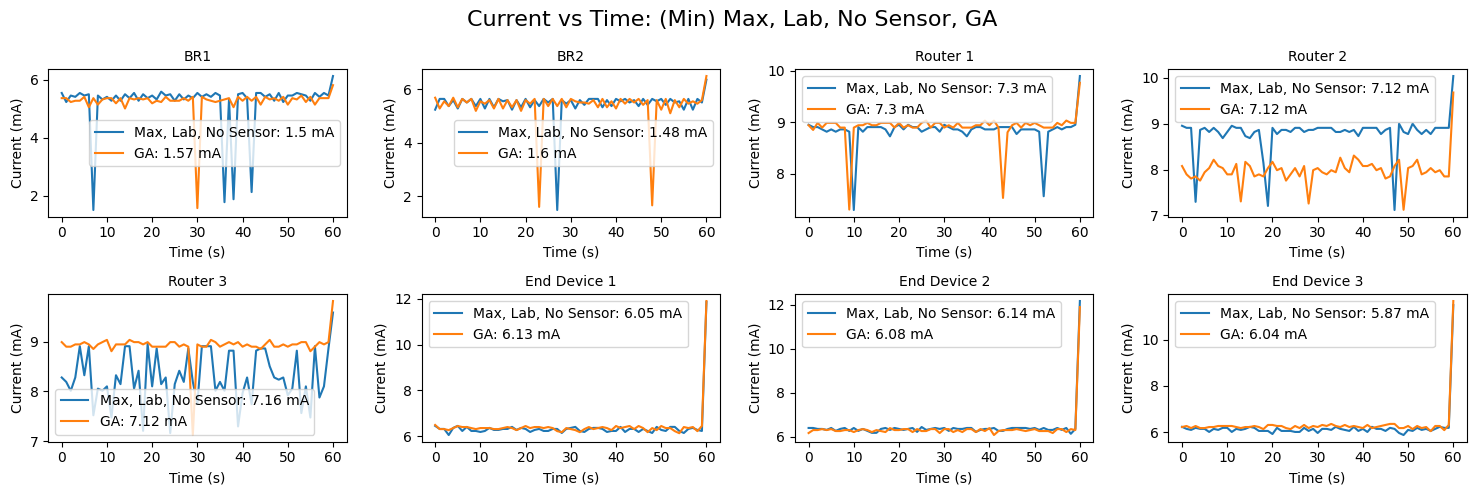
\includegraphics[width=1\textwidth]{images/research_results/current_consumption_analysis/optimized/lab/no_sensor/ga/comparison/min_comparison_lab_no-sensor_vs_lab_no-sensor_ga.png}
    \caption{Minimum Current Consumption Comparison in Lab location, No Sensor mode vs. Lab location, No Sensor mode, GA optimized mode.}
    \label{fig:min_comparison_lab_no-sensor_vs_lab_no-sensor_ga}
\end{figure}

The comparison graphs for Maximum and Optimized modes reveal significant differences in current consumption. The Optimized GA mode generally exhibits lower maximum, minimum, and mean current consumption for most devices. This is likely due to varying transmission power settings determined by the Genetic Algorithm.

\paragraph{Mode: Ping}
In the Ping mode, devices transmit data at varying intervals, with the ping frequency ranging from 50 in 60 seconds to 290 in 300 seconds, depending on the location. This analysis focuses on the active device mode when devices send pings.

\subparagraph{Monte Carlo Method}
The following plot and table illustrate the impact of this optimization technique on current consumption in the Monte Carlo Method (MCM), aiming to improve energy efficiency during active communication.

\begin{figure}[H]
  \centering
  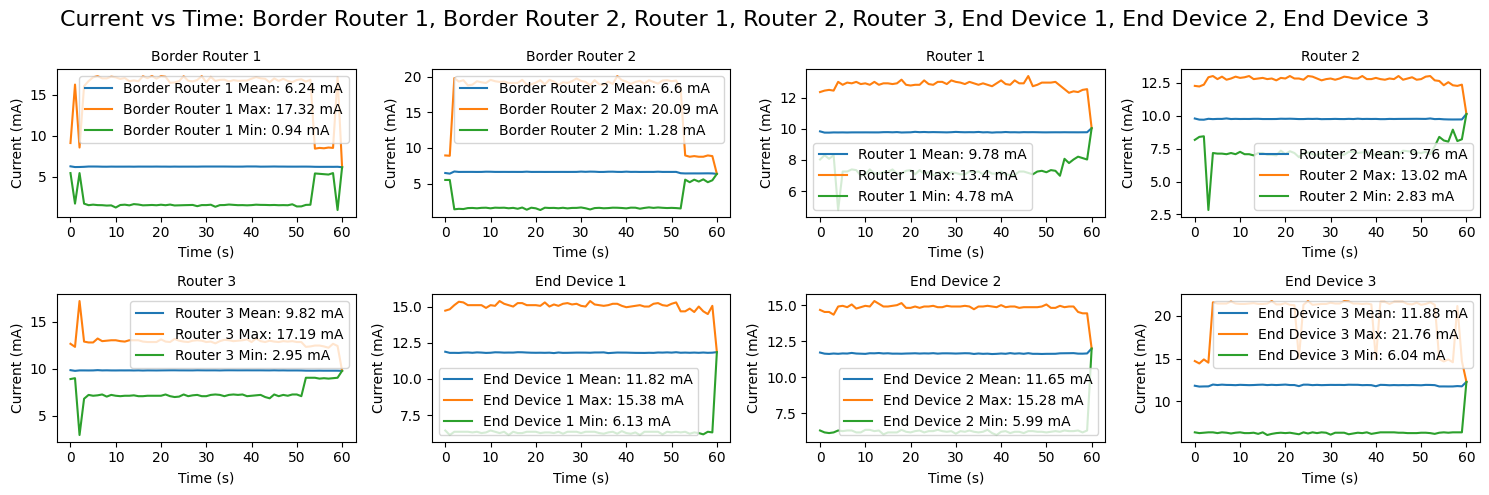
\includegraphics[width=1\textwidth]{images/research_results/current_consumption_analysis/optimized/lab/ping/mc/overview.png}
    \caption{Overview of Current Consumption in Lab location, Ping mode, MCM optimized mode.}
    \label{fig:overview_lab_ping_mc_overview}
\end{figure}

\begin{longtblr}[
  caption = {Current consumption overview from individual devices.},
  label = {tab:current_consumption_overview},
  ]{
  colspec = {X[l] X[l] X[l] X[l] X[l] X[l] X[l]},
  hlines, vlines,
  rowhead = 1, % Repeat the header row on every page
  row{1} = {font=\bfseries},
}
  Device & Input txpower $(dBm)$ & Total Ping & Mean $(mA)$ & Max $(mA)$ & Min $(mA)$ \\
  Border Router 1 & -8 & \SetCell[r=8]{c} 50 & 6.24 & 17.32 & 0.94 \\
  Border Router 2 & 8 &  & 6.6 & 20.09 & 1.28 \\
  Router 1 & -16 &  & 9.78 & 13.4 & 4.78 \\
  Router 2 & 0 &  & 9.76 & 13.02 & 2.83 \\
  Router 3 & 0 &  & 9.82 & 17.19 & 2.95 \\
  End device 1 & -8 &  & 11.82 & 15.38 & 6.13 \\
  End device 2 & -20 &  & 11.65 & 15.28 & 5.99 \\
  End device 3 & 8 &  & 11.88 & 21.76 & 6.04 \\
\end{longtblr}

\subparagraph{Comparison: Maximum Lab Ping vs Optimized Lab Ping MCM}
The following plots provide a comparison analysis between Maximum and Optimized MCM modes to evaluate the power consumption differences and potential improvements in energy efficiency.

\begin{figure}[H]
  \centering
  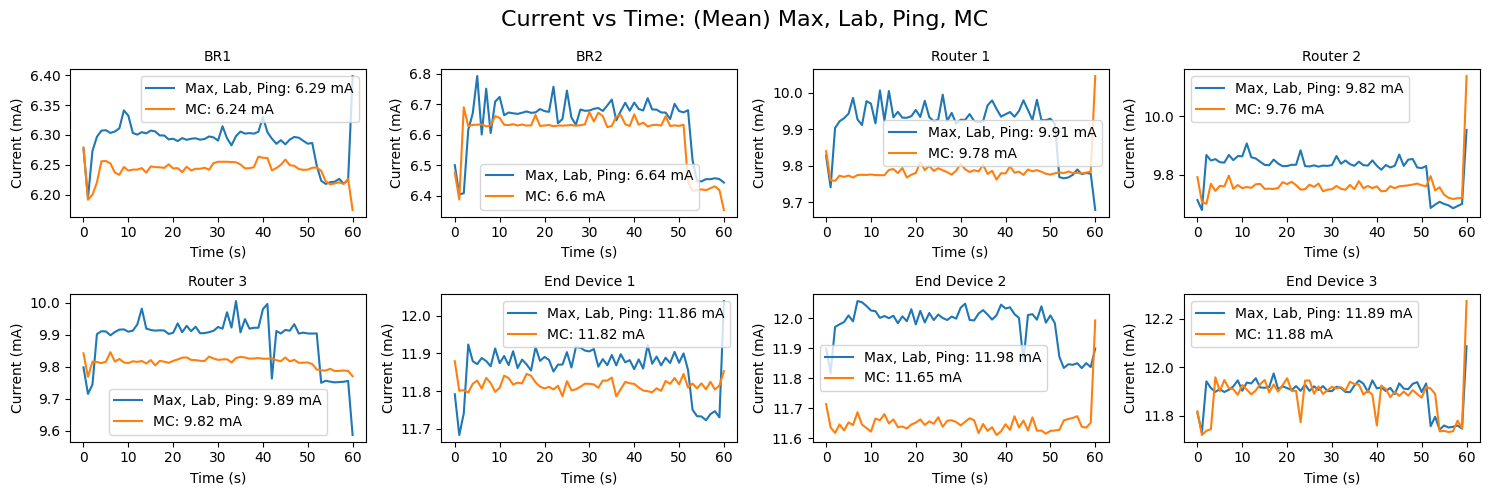
\includegraphics[width=1\textwidth]{images/research_results/current_consumption_analysis/optimized/lab/ping/mc/comparison/mean_comparison_lab_ping_mc_vs_lab_ping_mc.png}
    \caption{Mean Current Consumption Comparison in Lab location, Ping mode, MCM optimized mode vs. Lab location, Ping mode, MCM optimized mode.}
    \label{fig:mean_comparison_lab_ping_mc_vs_lab_ping_mc}
\end{figure}

\begin{figure}[H]
  \centering
  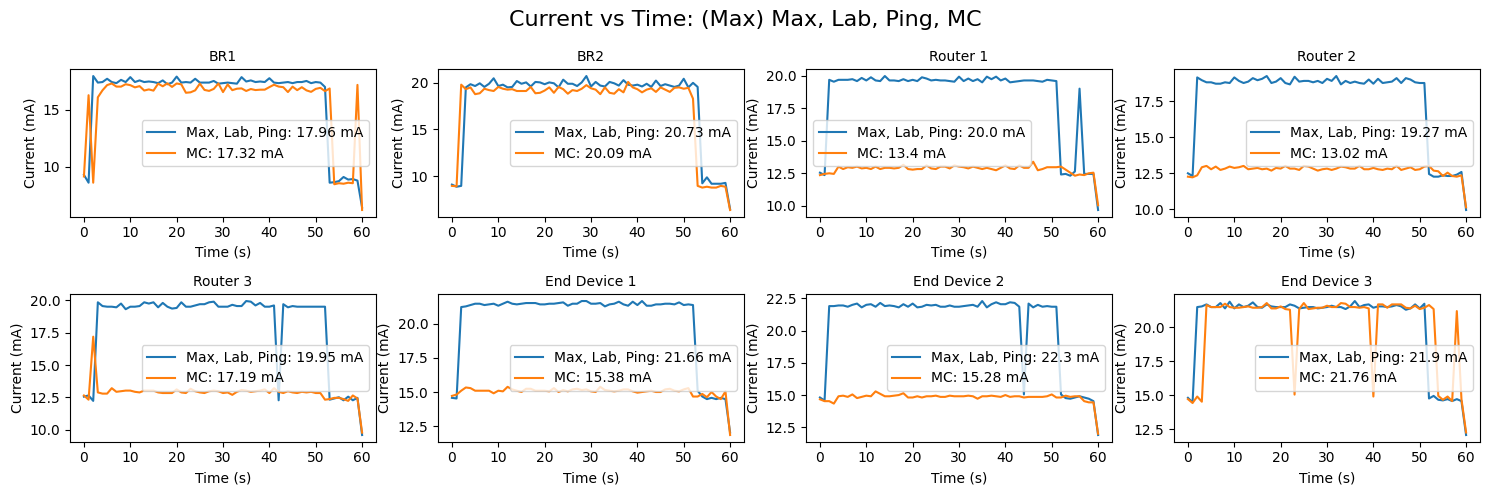
\includegraphics[width=1\textwidth]{images/research_results/current_consumption_analysis/optimized/lab/ping/mc/comparison/max_comparison_lab_ping_mc_vs_lab_ping_mc.png}
    \caption{Maximum Current Consumption Comparison in Lab location, Ping mode, MCM optimized mode vs. Lab location, Ping mode, MCM optimized mode.}
    \label{fig:max_comparison_lab_ping_mc_vs_lab_ping_mc}
\end{figure}

\begin{figure}[H]
  \centering
  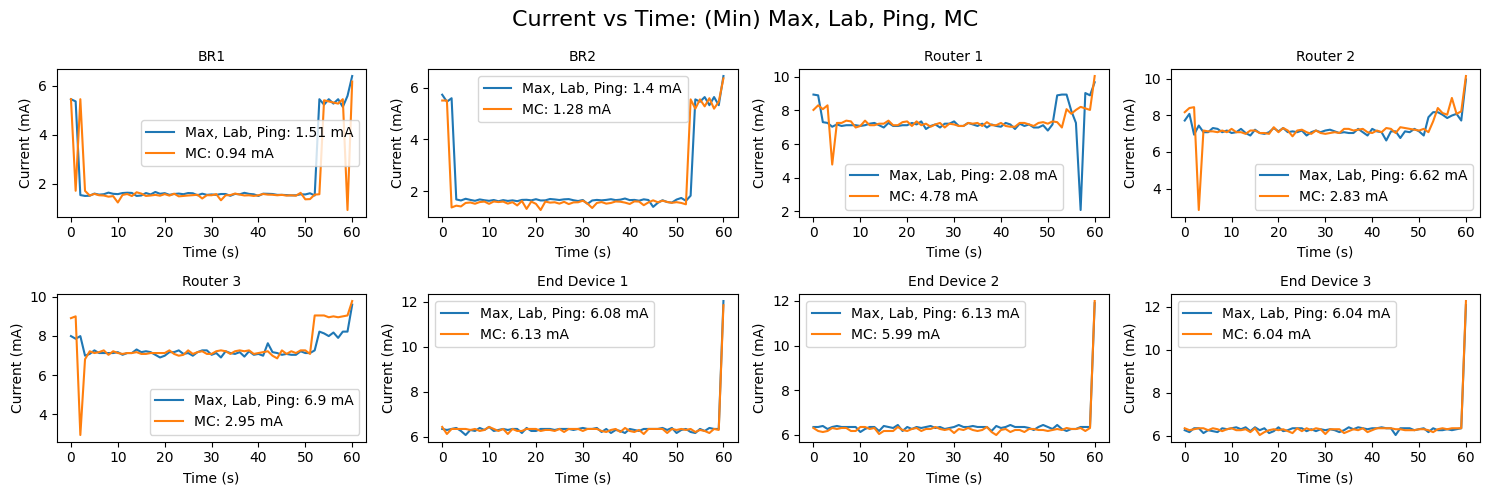
\includegraphics[width=1\textwidth]{images/research_results/current_consumption_analysis/optimized/lab/ping/mc/comparison/min_comparison_lab_ping_mc_vs_lab_ping_mc.png}
    \caption{Minimum Current Consumption Comparison in Lab location, Ping mode, MCM optimized mode vs. Lab location, Ping mode, MCM optimized mode.}
    \label{fig:min_comparison_lab_ping_mc_vs_lab_ping_mc}
\end{figure}

The comparison graphs present the optimized mode demonstrating lower mean current consumption values for several devices, particularly in the case of Router 1, Router 2, and End device 2. The maximum current consumption values are also notably lower in the optimized mode for some devices, highlighting the benefits of power optimization in improving the overall network performance and energy efficiency.

\subparagraph{Genetic Algorithm}
The following plot and table showcase the differences in current consumption resulting from using a Genetic Algorithm (GA), which aims to reduce power consumption and improve overall energy efficiency.

\begin{figure}[H]
  \centering
  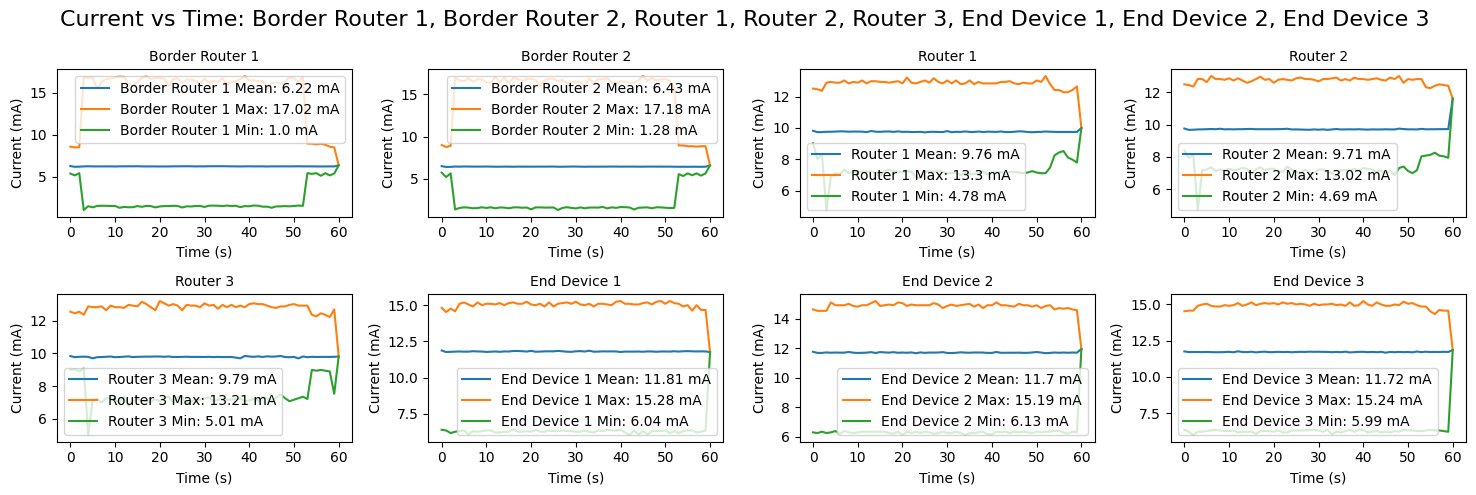
\includegraphics[width=1\textwidth]{images/research_results/current_consumption_analysis/optimized/lab/ping/ga/overview.png}
    \caption{Overview of Current Consumption in Lab location, Ping mode, GA optimized mode.}
    \label{fig:overview_lab_ping_ga_overview}
\end{figure}

\begin{longtblr}[
  caption = {Overview of Current Consumption in Lab location, Ping mode, GA optimized mode.},
  label = {tab:overview_lab_ping_ga_overview},
  ]{
  colspec = {X[l] X[l] X[l] X[l] X[l] X[l] X[l]},
  hlines, vlines,
  rowhead = 1, % Repeat the header row on every page
  row{1} = {font=\bfseries},
}
  Device & Input txpower $(dBm)$ & Total Ping & Mean $(mA)$ & Max $(mA)$ & Min $(mA)$ \\
  Border Router 1 & \SetCell[r=8]{c} -20 & \SetCell[r=8]{c} 50 & 6.22 & 17.02 & 1.0 \\
  Border Router 2 &  &  & 6.43 & 17.18 & 1.28 \\
  Router 1 &  &  & 9.76 & 13.3 & 4.78 \\
  Router 2 &  &  & 9.71 & 13.02 & 4.69 \\
  Router 3 &  &  & 9.79 & 13.21 & 5.01 \\
  End device 1 &  &  & 11.81 & 15.28 & 6.04 \\
  End device 2 &  &  & 11.7 & 15.19 & 6.13 \\
  End device 3 &  &  & 11.72 & 15.24 & 5.99 \\
\end{longtblr}

\subparagraph{Comparison: Optimized Lab Ping MCM vs Optimized Lab Ping GA}
The following comparison plots represent the differences in current consumption between the MCM and GA modes from the exact location, showcasing the impact of the Monte Carlo Method and Genetic Algorithm optimization approaches.

\begin{figure}[H]
  \centering
  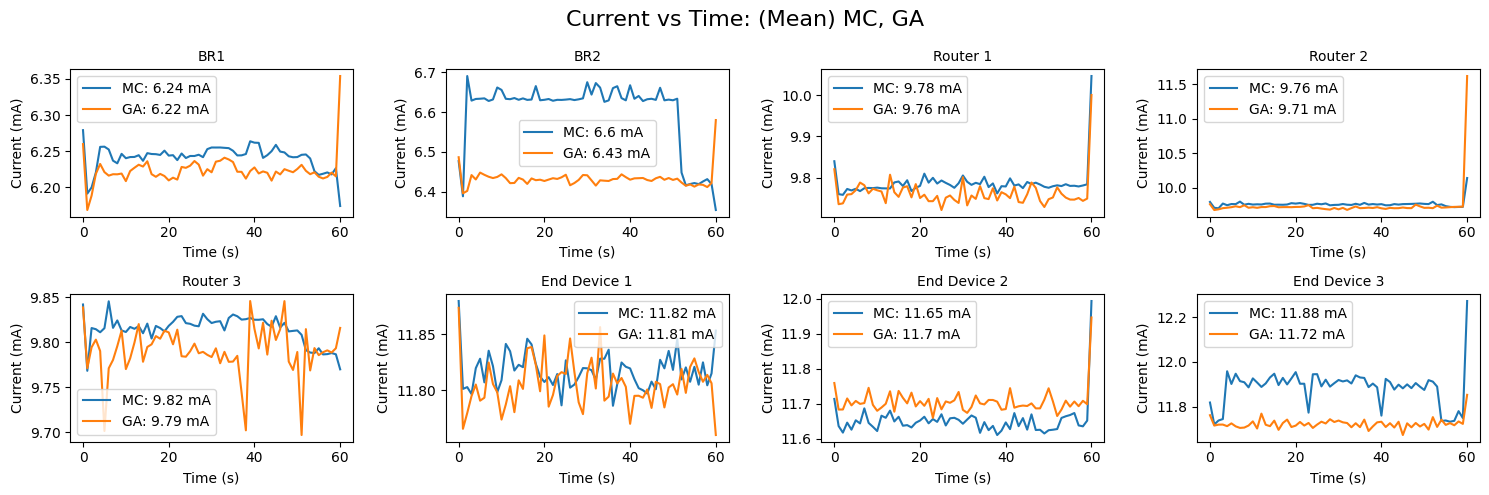
\includegraphics[width=1\textwidth]{images/research_results/current_consumption_analysis/optimized/lab/ping/ga/comparison/mean_comparison_lab_ping_mc_vs_lab_ping_ga.png}
    \caption{Mean Current Consumption Comparison in Lab location, Ping mode, MCM optimized mode vs. Lab location, Ping mode, GA optimized mode.}
    \label{fig:mean_comparison_lab_ping_mc_vs_lab_ping_ga}
\end{figure}

\begin{figure}[H]
  \centering
  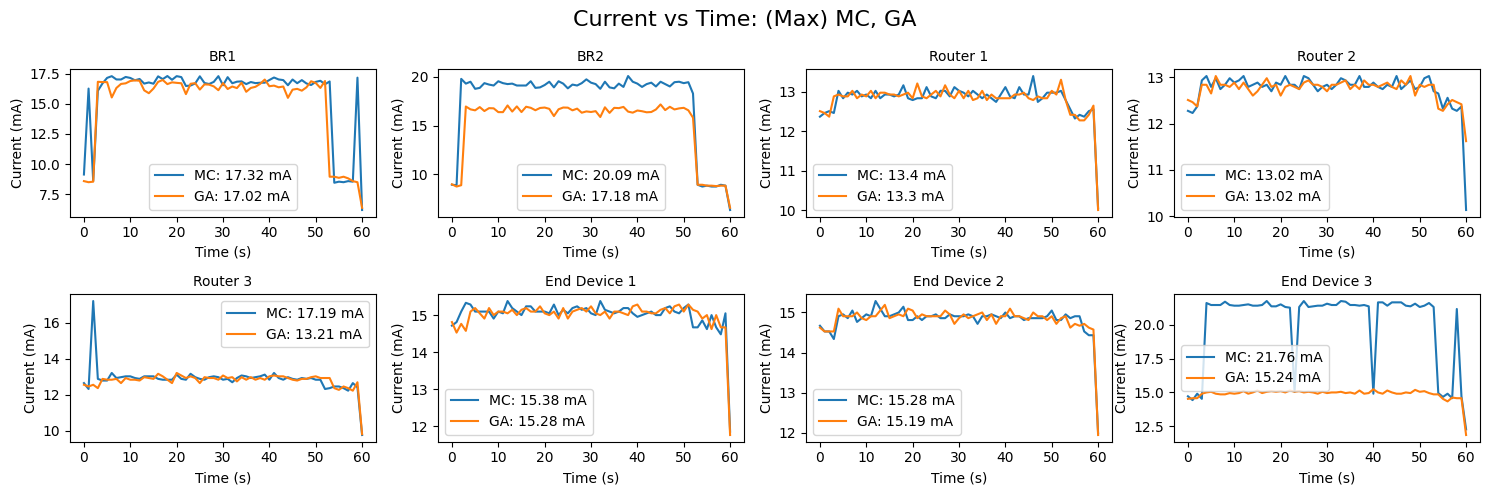
\includegraphics[width=1\textwidth]{images/research_results/current_consumption_analysis/optimized/lab/ping/ga/comparison/max_comparison_lab_ping_mc_vs_lab_ping_ga.png}
    \caption{Maximum Current Consumption Comparison in Lab location, Ping mode, MCM optimized mode vs. Lab location, Ping mode, GA optimized mode.}
    \label{fig:max_comparison_lab_ping_mc_vs_lab_ping_ga}
\end{figure}

\begin{figure}[H]
  \centering
  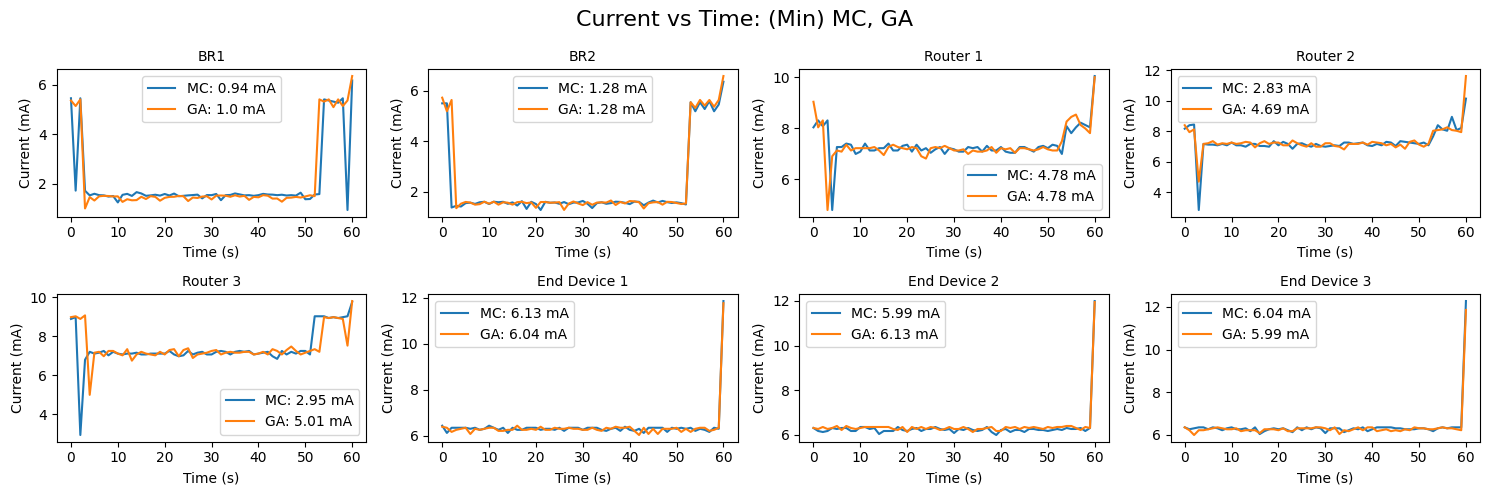
\includegraphics[width=1\textwidth]{images/research_results/current_consumption_analysis/optimized/lab/ping/ga/comparison/min_comparison_lab_ping_mc_vs_lab_ping_ga.png}
    \caption{Minimum Current Consumption Comparison in Lab location, Ping mode, MCM optimized mode vs. Lab location, Ping mode, GA optimized mode.}
    \label{fig:min_comparison_lab_ping_mc_vs_lab_ping_ga}
\end{figure}

The graphs comparing Optimized Lab Ping MC and GA modes reveal differences in device performance under these optimization methods. Generally, Optimized Lab Ping GA mode yields slightly lower mean current consumption for most devices and reduced maximum current consumption for some devices, while minimum Current consumption results vary. The GA mode consistently uses -20 dBm transmission power, while the MCM mode varies. This difference may influence current consumption patterns.


\subsubsection{Location: Home}
This section examines the more considerable device distances and 300 seconds of data compared to the lab's 60 seconds. The accompanying plot and table reveal the impact of these factors on the network's current consumption.

\paragraph{Mode: No Sensor}
This section showcases the current consumption in No Sensor mode, where devices are idle and not actively sending pings. The data highlights the impact of the increased distance between devices on power consumption in this mode.

\subparagraph{Monte Carlo Method}
The following plot and table provide an overview of the current consumption for each device in the network, showcasing the impact of the Monte Carlo Method (MCM) on power usage.

\begin{figure}[H]
  \centering
  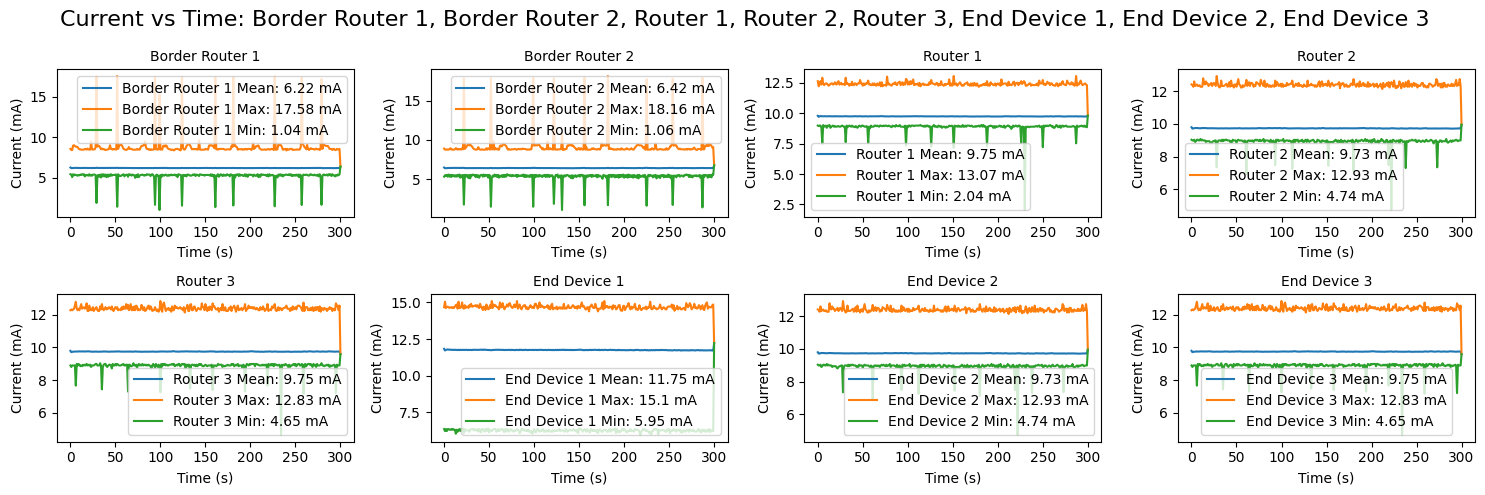
\includegraphics[width=1\textwidth]{images/research_results/current_consumption_analysis/optimized/home/no_sensor/mc/overview.png}
    \caption{Overview of Current Consumption in Home location, No Sensor mode, MCM optimized mode.}
    \label{fig:overview_home_no_sensor_mc_overview}
\end{figure}

\begin{longtblr}[
  caption = {Overview of Current Consumption in Home location, No Sensor mode, MCM optimized mode.},
  label = {tab:overview_home_no_sensor_mc_overview},
  ]{
  colspec = {X[l] X[l] X[l] X[l] X[l] X[l] X[l]},
  hlines, vlines,
  rowhead = 1, % Repeat the header row on every page
  row{1} = {font=\bfseries},
}
  Device & Input txpower & Total Ping & Mean $(mA)$ & Max $(mA)$ & Min $(mA)$ \\
  Border Router 1 & 8 & \SetCell[r=8]{c} 0 & 6.22 & 17.58 & 1.04 \\
  Border Router 2 & 8 &  & 6.42 & 18.16 & 1.06 \\
  Router 1 & -8 &  & 9.75 & 13.07 & 2.04 \\
  Router 2 & -20 &  & 9.73 & 12.93 & 4.74 \\
  Router 3 & -4 &  & 9.75 & 12.83 & 4.65 \\
  End device 1 & -16 &  & 11.75 & 15.1 & 5.95 \\
  End device 2 & 4 &  & 9.73 & 12.93 & 4.74 \\
  End device 3 & -16 &  & 9.75 & 12.83 & 4.65 \\
\end{longtblr}

\subparagraph{Comparison: Home - Maximum No Sensor vs Optimized No Sensor MCM}
The following comparison graphs depict the differences between Maximum and Optimized No Sensor MCM modes in the home environment, focusing on each device's varying transmission power settings.

\begin{figure}[H]
  \centering
  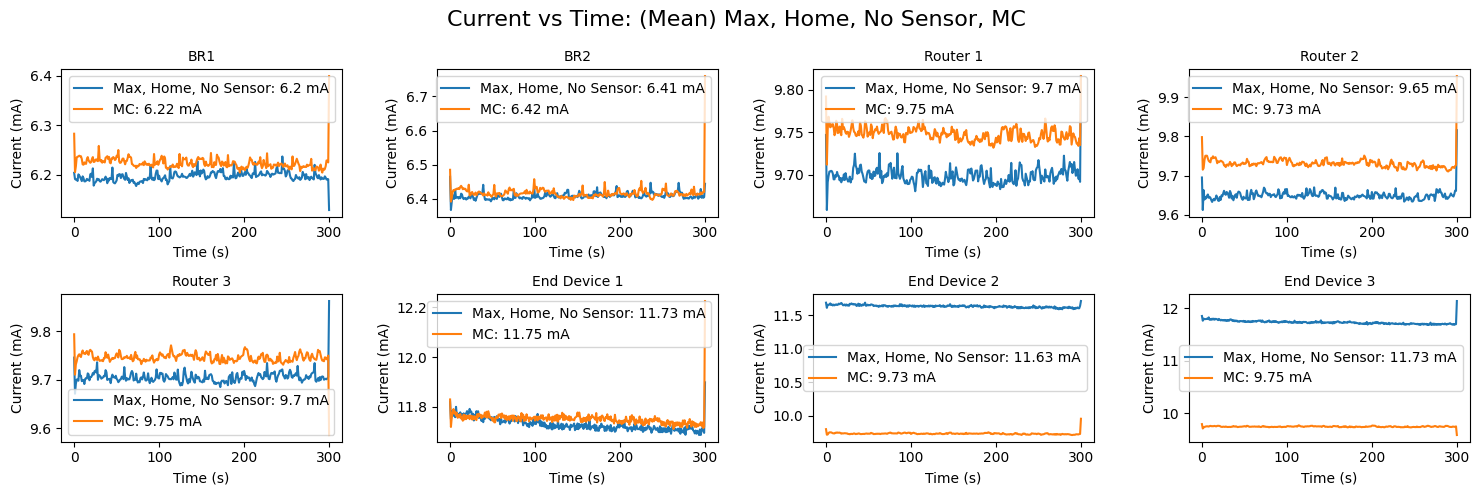
\includegraphics[width=1\textwidth]{images/research_results/current_consumption_analysis/optimized/home/no_sensor/mc/comparison/mean_comparison_home_no_sensor_mc_vs_home_no_sensor_max.png}
    \caption{Mean Current Consumption Comparison in Home location, No Sensor mode, MCM optimized mode vs. Home location, No Sensor mode, Maximum mode.}
    \label{fig:mean_comparison_home_no_sensor_mc_vs_home_no_sensor_max}
\end{figure}

\begin{figure}[H]
  \centering
  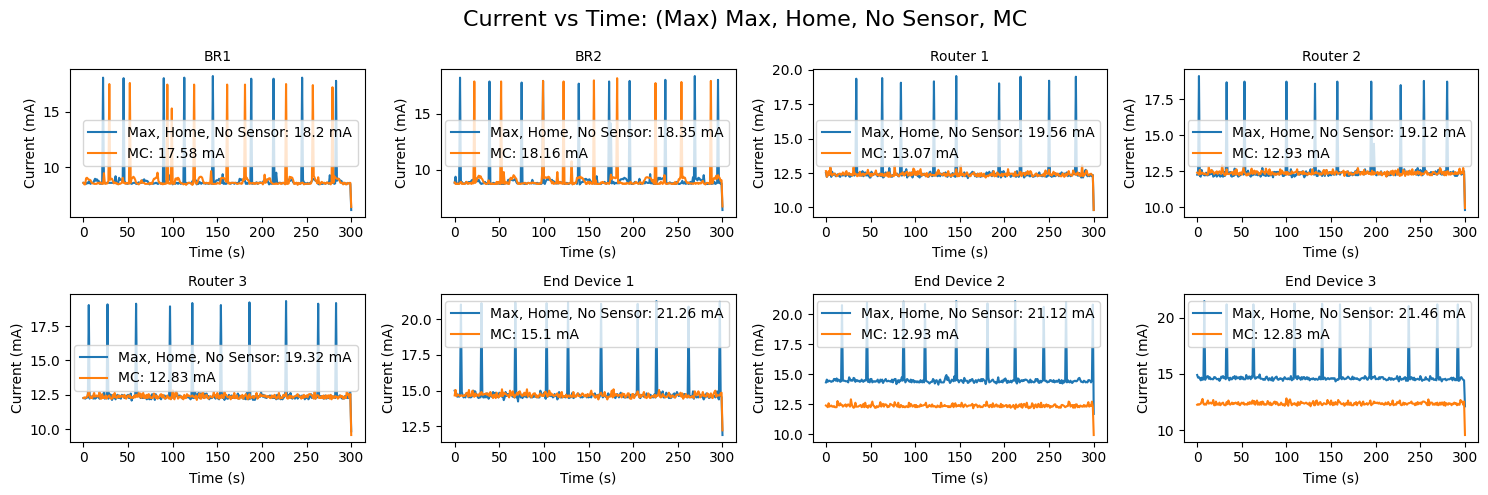
\includegraphics[width=1\textwidth]{images/research_results/current_consumption_analysis/optimized/home/no_sensor/mc/comparison/max_comparison_home_no_sensor_mc_vs_home_no_sensor_max.png}
    \caption{Maximum Current Consumption Comparison in Home location, No Sensor mode, MCM optimized mode vs. Home location, No Sensor mode, Maximum mode.}
    \label{fig:max_comparison_home_no_sensor_mc_vs_home_no_sensor_max}
\end{figure}

\begin{figure}[H]
  \centering
  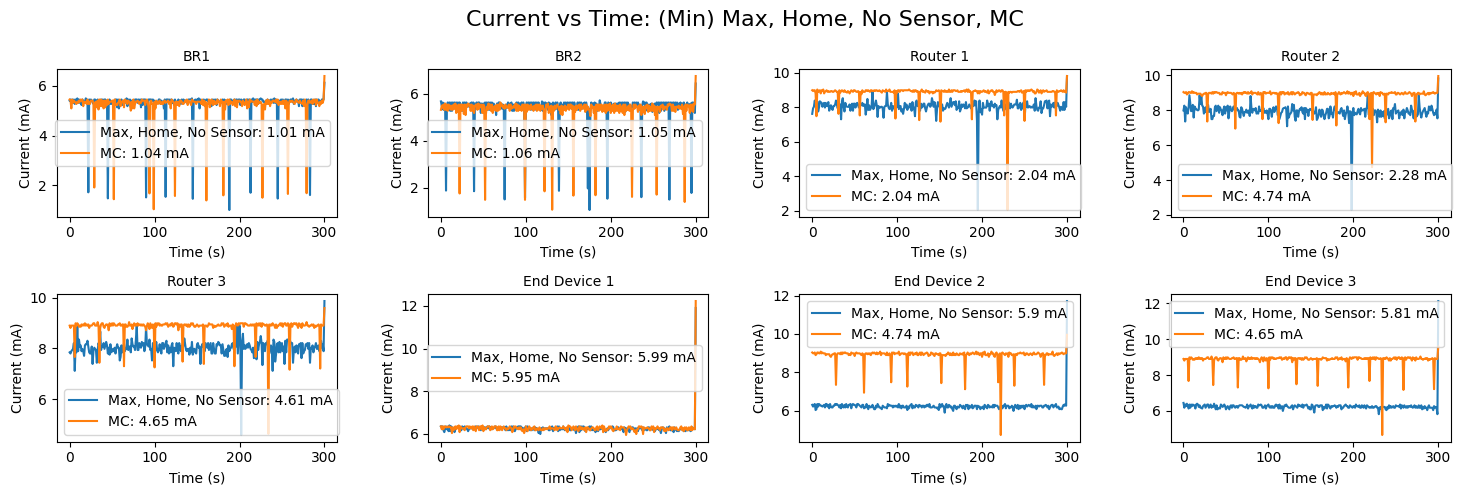
\includegraphics[width=1\textwidth]{images/research_results/current_consumption_analysis/optimized/home/no_sensor/mc/comparison/min_comparison_home_no_sensor_mc_vs_home_no_sensor_max.png}
    \caption{Minimum Current Consumption Comparison in Home location, No Sensor mode, MCM optimized mode vs. Home location, No Sensor mode, Maximum mode.}
    \label{fig:min_comparison_home_no_sensor_mc_vs_home_no_sensor_max}
\end{figure}

The comparison graphs reveal differences in current consumption between Maximum and Optimized MCM modes. Border Routers 1 and 2 show slightly higher mean current values in Maximum mode, while Routers 1, 2, and 3 exhibits marginally lower values. End Devices 1, 2, and 3 have higher mean current values in the Maximum mode. Overall, the Maximum mode has slightly increased current consumption compared to the Optimized MCM mode, but the differences are insignificant.

\subparagraph{Genetic Algorithm}
The following plot and table present the current consumption overview of each device in the network, utilizing Genetic Algorithm (GA) optimized transmission power settings.

\begin{figure}[H]
  \centering
  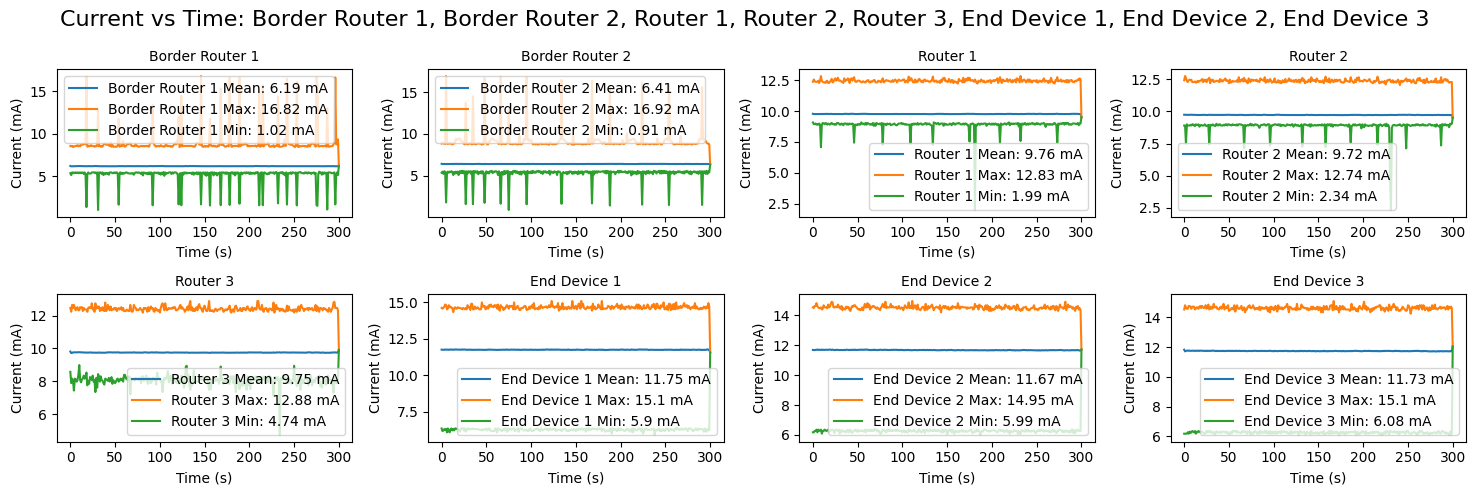
\includegraphics[width=1\textwidth]{images/research_results/current_consumption_analysis/optimized/home/no_sensor/ga/overview.png}
    \caption{Overview of Current Consumption in Home location, No Sensor mode, GA optimized mode.}
    \label{fig:overview_home_no_sensor_ga_overview}
\end{figure}

\begin{longtblr}[
  caption = {Overview of Current Consumption in Home location, No Sensor mode, GA optimized mode.},
  label = {tab:overview_home_no_sensor_ga_overview},
  ]{
  colspec = {X[l] X[l] X[l] X[l] X[l] X[l] X[l]},
  hlines, vlines,
  rowhead = 1, % Repeat the header row on every page
  row{1} = {font=\bfseries},
}
  Device & Input txpower & Total Ping & Mean $(mA)$ & Max $(mA)$ & Min $(mA)$ \\
  Border Router 1 & -20 & \SetCell[r=8]{c} 0 & 6.19 & 16.82 & 1.02 \\
  Border Router 2 & -19 &  & 6.41 & 16.92 & 0.91 \\
  Router 1 & -19 &  & 9.76 & 12.83 & 1.99 \\
  Router 2 & -20 &  & 9.72 & 12.74 & 2.34 \\
  Router 3 & -18 &  & 9.75 & 12.88 & 4.74 \\
  End device 1 & -18 &  & 11.75 & 15.1 & 5.9 \\
  End device 2 & -16 &  & 11.67 & 14.95 & 5.99 \\
  End device 3 & -19 &  & 11.73 & 15.1 & 6.08 \\
\end{longtblr}

\subparagraph{Comparison: Optimized Home No Sensor: MCM vs GA}
The following comparison graphs showcase the differences in current consumption between the Monte Carlo Method (MCM) and Genetic Algorithm (GA) optimization techniques for the No Sensor mode.

\begin{figure}[H]
  \centering
  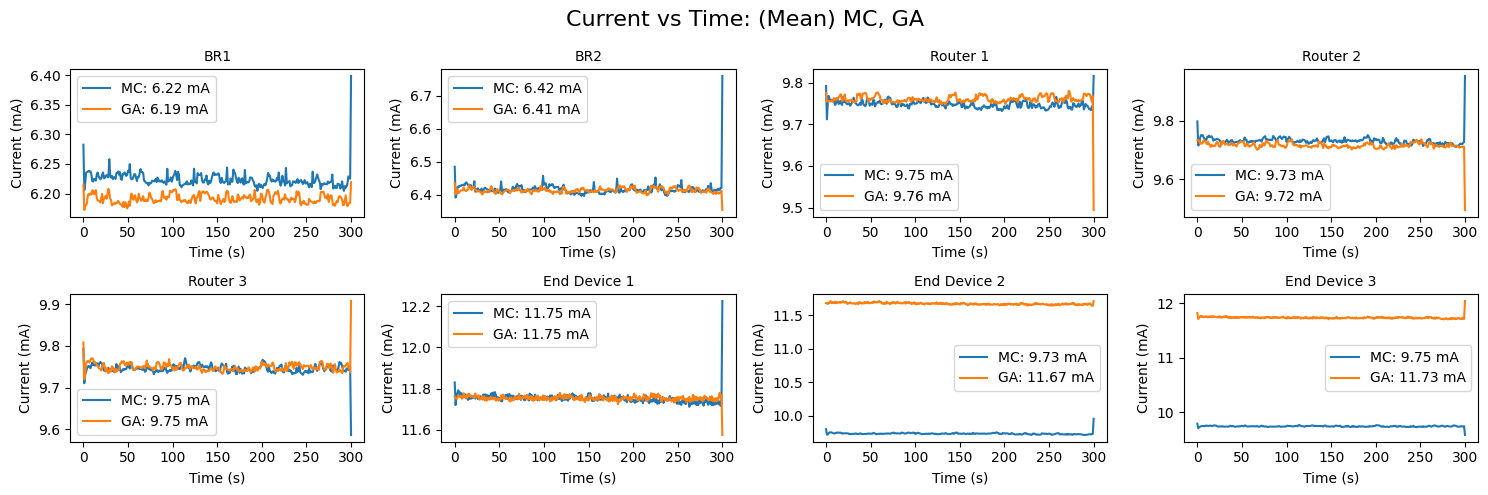
\includegraphics[width=1\textwidth]{images/research_results/current_consumption_analysis/optimized/home/no_sensor/ga/comparison/mean_comparison_home_no_sensor_ga_vs_home_no_sensor_mc.png}
    \caption{Mean Current Consumption Comparison in Home location, No Sensor mode, GA optimized mode vs. Home location, No Sensor mode, MCM optimized mode.}
    \label{fig:mean_comparison_home_no_sensor_ga_vs_home_no_sensor_mc}
\end{figure}

\begin{figure}[H]
  \centering
  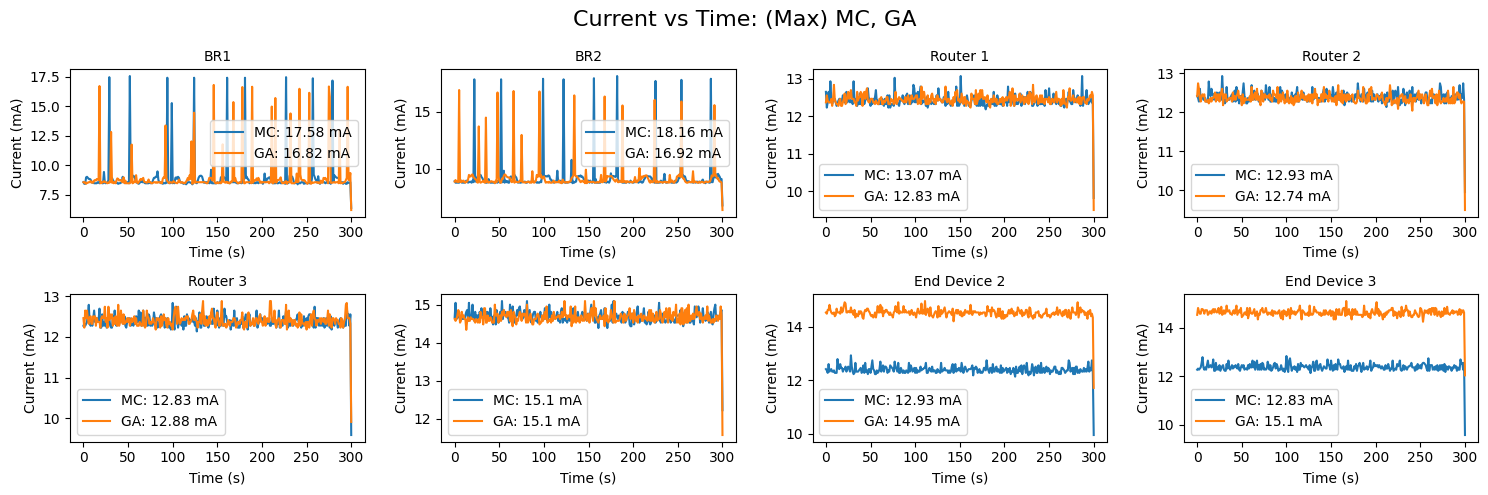
\includegraphics[width=1\textwidth]{images/research_results/current_consumption_analysis/optimized/home/no_sensor/ga/comparison/max_comparison_home_no_sensor_ga_vs_home_no_sensor_mc.png}
    \caption{Maximum Current Consumption Comparison in Home location, No Sensor mode, GA optimized mode vs. Home location, No Sensor mode, MCM optimized mode.}
    \label{fig:max_comparison_home_no_sensor_ga_vs_home_no_sensor_mc}
\end{figure}

\begin{figure}[H]
  \centering
  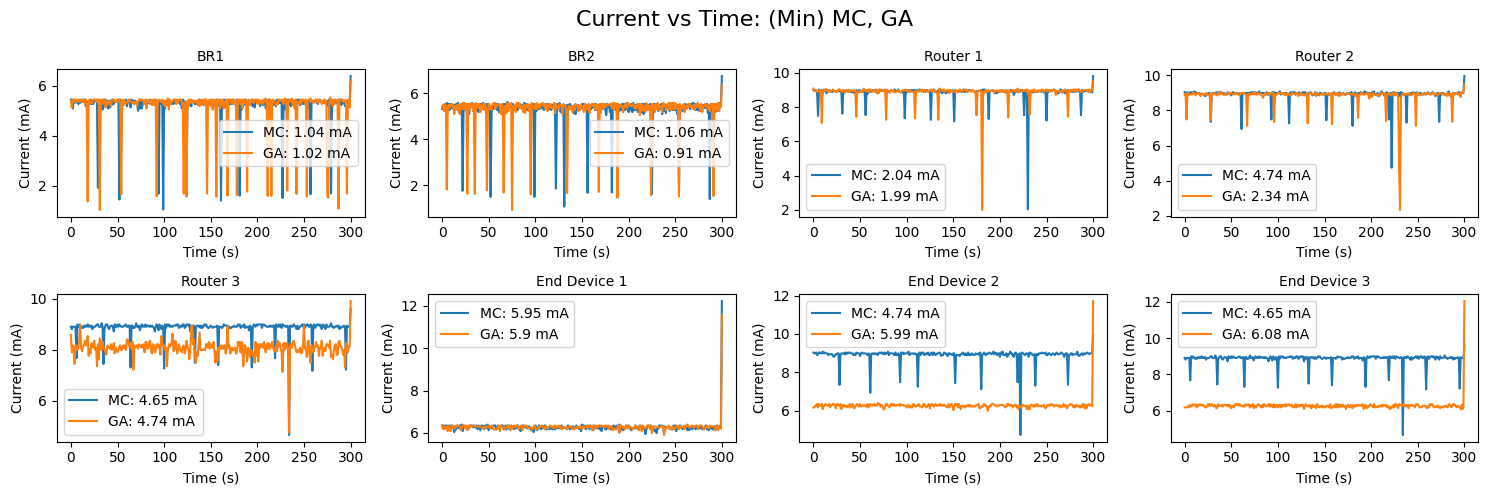
\includegraphics[width=1\textwidth]{images/research_results/current_consumption_analysis/optimized/home/no_sensor/ga/comparison/min_comparison_home_no_sensor_ga_vs_home_no_sensor_mc.png}
    \caption{Minimum Current Consumption Comparison in Home location, No Sensor mode, GA optimized mode vs. Home location, No Sensor mode, MCM optimized mode.}
    \label{fig:min_comparison_home_no_sensor_ga_vs_home_no_sensor_mc}
\end{figure}

The comparison graphs depict the differences in input transmission power, mean current, maximum current, and minimum current for each device in the MCM and GA modes. Border Routers and Routers have slightly lower mean current values in GA mode, while End Devices show similar values across both modes. The current consumption between MC and GA modes is similar, with minor device variations.

\paragraph{Mode: Ping}
This section presents the current consumption in ping mode, aiming to evaluate the performance of devices in the network while the radio is active.

\subparagraph{Monte Carlo Method}
The plot and table showcase the current consumption overview for each device in the network, highlighting the impact of the Monte Carlo optimization method.

\begin{figure}[H]
  \centering
  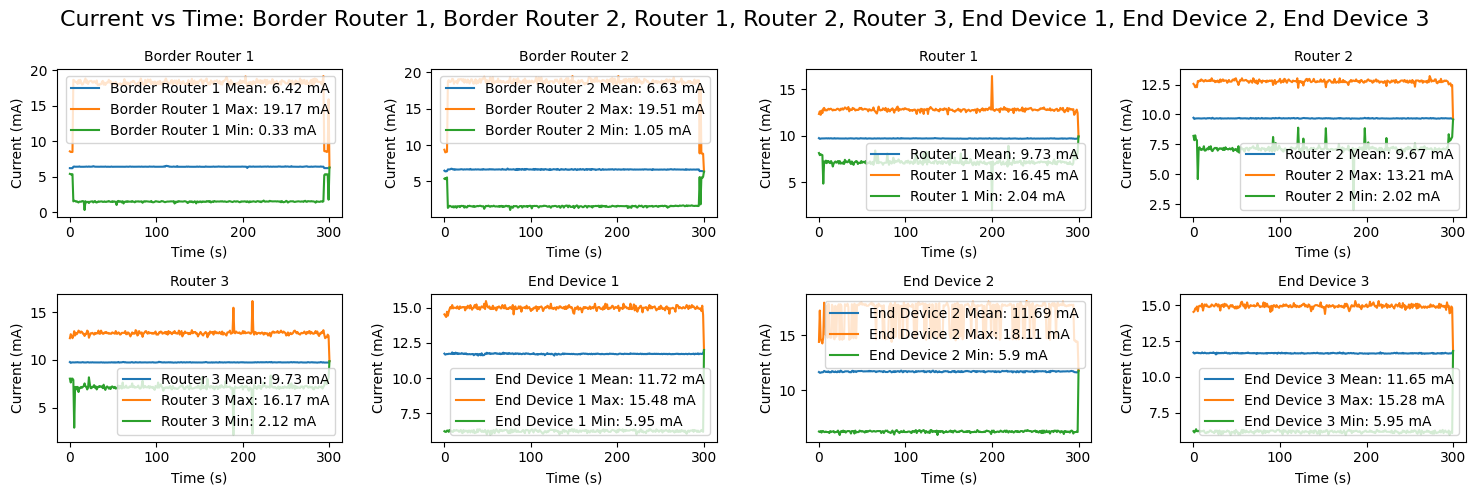
\includegraphics[width=1\textwidth]{images/research_results/current_consumption_analysis/optimized/home/ping/mc/overview.png}
    \caption{Overview of Current Consumption in Home location, Ping mode, MCM optimized mode.}
    \label{fig:overview_home_ping_mc_overview}
\end{figure}

\begin{longtblr}[
  caption = {Overview of Current Consumption in Home location, Ping mode, MCM optimized mode.},
  label = {tab:overview_home_ping_mc_overview},
  ]{
  colspec = {X[l] X[l] X[l] X[l] X[l] X[l] X[l]},
  hlines, vlines,
  rowhead = 1, % Repeat the header row on every page
  row{1} = {font=\bfseries},
}
  Device & Input txpower & Total Ping & Mean $(mA)$ & Max $(mA)$ & Min $(mA)$ \\
  Border Router 1 & 8 & \SetCell[r=8]{c} 290 & 6.42 & 19.17 & 0.33 \\
  Border Router 2 & 8 &  & 6.63 & 19.51 & 1.05 \\
  Router 1 & -8 &  & 9.73 & 16.45 & 2.04 \\
  Router 2 & -20 &  & 9.67 & 13.21 & 2.02 \\
  Router 3 & -4 &  & 9.73 & 16.17 & 2.12 \\
  End device 1 & -16 &  & 11.72 & 15.48 & 5.95 \\
  End device 2 & 4 &  & 11.69 & 18.11 & 5.9 \\
  End device 3 & -16 &  & 11.65 & 15.28 & 5.95 \\
\end{longtblr}

\subparagraph{Comparison: Optimized Ping MCM - Lab vs Home}
The following comparison graphs showcase the differences in current consumption between the two locations using the Monte Carlo Method (MCM) optimization.

\begin{figure}[H]
  \centering
  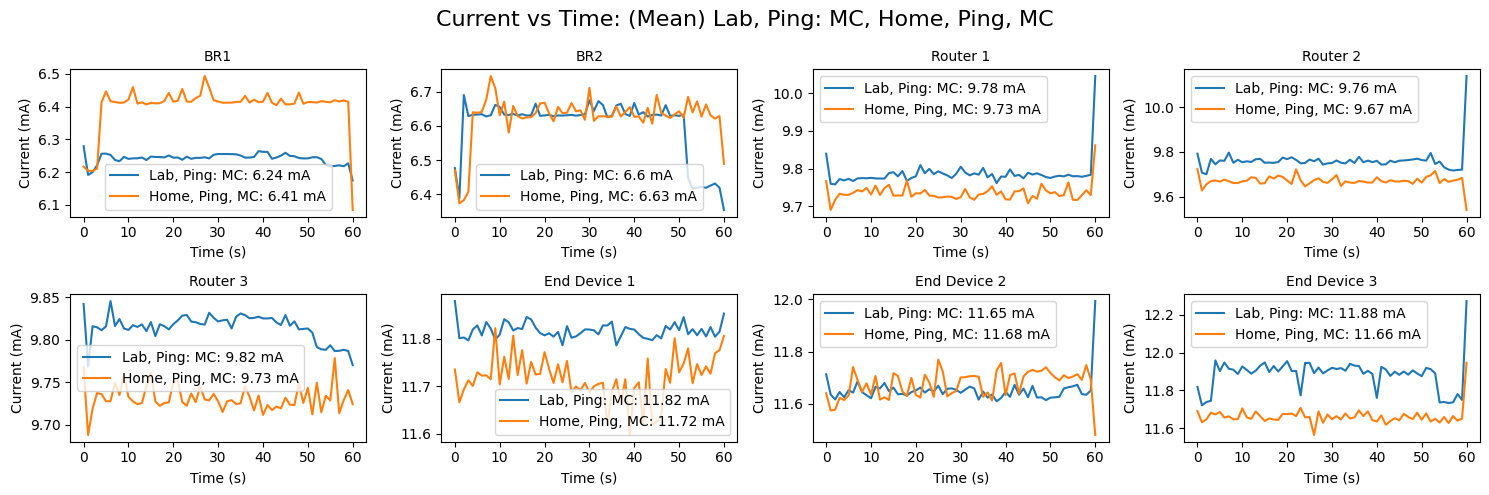
\includegraphics[width=1\textwidth]{images/research_results/current_consumption_analysis/optimized/home/ping/mc/comparison/mean_comparison_home_ping_mc_vs_lab_ping_mc.png}
    \caption{Mean Current Consumption Comparison in Home location, Ping mode, MCM optimized mode vs. Lab location, Ping mode, MCM optimized mode.}
    \label{fig:mean_comparison_home_ping_mc_vs_lab_ping_mc}
\end{figure}

\begin{figure}[H]
  \centering
  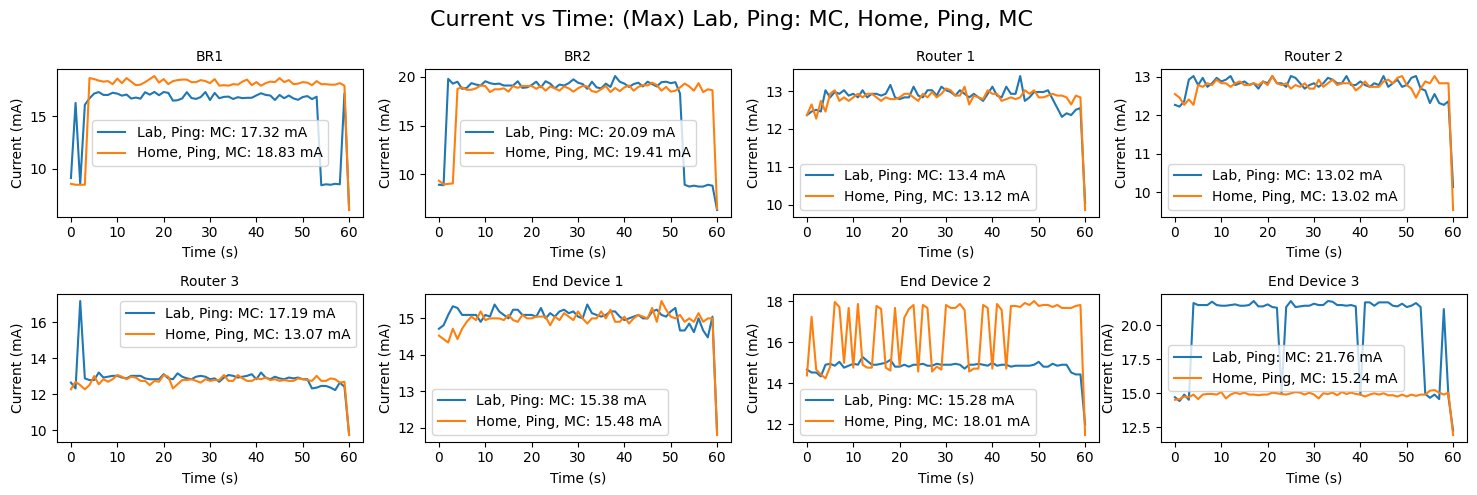
\includegraphics[width=1\textwidth]{images/research_results/current_consumption_analysis/optimized/home/ping/mc/comparison/max_comparison_home_ping_mc_vs_lab_ping_mc.png}
    \caption{Maximum Current Consumption Comparison in Home location, Ping mode, MCM optimized mode vs. Lab location, Ping mode, MCM optimized mode.}
    \label{fig:max_comparison_home_ping_mc_vs_lab_ping_mc}
\end{figure}

\begin{figure}[H]
  \centering
  \includegraphics[width=1\textwidth]{images/research_results/current_consumption_analysis/optimized/home/ping/mc/comparison/min_comparison_home_ping_mc_vs_lab_ping_mc.png}
    \caption{Minimum Current Consumption Comparison in Home location, Ping mode, MCM optimized mode vs. Lab location, Ping mode, MCM optimized mode.}
    \label{fig:min_comparison_home_ping_mc_vs_lab_ping_mc}
\end{figure}

Considering that the Home environment has a greater distance between devices than the Lab environment, the data comparison shows that the MCM modes demonstrate robust performance in both settings. Despite the increased distance in the Home environment, the mean current values for Routers and End Devices are reasonably close to those observed in the Lab environment. This indicates that the MCM mode effectively adjusts to various scenarios with different distances between devices and maintains consistent performance levels.

\subparagraph{Comparison: Maximum Home Ping vs Optimized Home Ping MCM}
The following comparison graphs showcase the differences in current consumption between the Maximum and Optimized Monte Carlo Methods (MCM) for optimization while the radio is active.

\begin{figure}[H]
  \centering
  \includegraphics[width=1\textwidth]{images/research_results/current_consumption_analysis/optimized/home/ping/mc/comparison/mean_comparison_home_ping_max_vs_home_ping_mc.png}
    \caption{Mean Current Consumption Comparison in Home location, Ping mode, Maximum MCM optimized mode vs. Home location, Ping mode, MCM optimized mode.}
    \label{fig:mean_comparison_home_ping_max_vs_home_ping_mc}
\end{figure}

\begin{figure}[H]
  \centering
  \includegraphics[width=1\textwidth]{images/research_results/current_consumption_analysis/optimized/home/ping/mc/comparison/max_comparison_home_ping_max_vs_home_ping_mc.png}
    \caption{Maximum Current Consumption Comparison in Home location, Ping mode, Maximum MCM optimized mode vs. Home location, Ping mode, MCM optimized mode.}
    \label{fig:max_comparison_home_ping_max_vs_home_ping_mc}
\end{figure}

\begin{figure}[H]
  \centering
  \includegraphics[width=1\textwidth]{images/research_results/current_consumption_analysis/optimized/home/ping/mc/comparison/min_comparison_home_ping_max_vs_home_ping_mc.png}
    \caption{Minimum Current Consumption Comparison in Home location, Ping mode, Maximum MCM optimized mode vs. Home location, Ping mode, MCM optimized mode.}
    \label{fig:min_comparison_home_ping_max_vs_home_ping_mc}
\end{figure}

The comparison graphs present the Optimized MCM mode demonstrates lower mean current values for Routers and End Devices when compared to the Maximum mode. Notably, the maximum current values for devices in the Maximum mode are consistently higher than those in the Optimized mode. The reduced mean and maximum current values in the Optimized mode indicate better energy efficiency and overall performance than in the Maximum mode.

\subparagraph{Genetic Algorithm}
The following plot and table illustrate the impact of current consumption for each device in the network when using GA optimization for transmission power settings while the radio is active.

\begin{figure}[H]
  \centering
  \includegraphics[width=1\textwidth]{images/research_results/current_consumption_analysis/optimized/home/ping/ga/overview.png}
    \caption{Overview of Current Consumption in Home location, Ping mode, GA optimized mode.}
    \label{fig:overview_home_ping_ga_overview}
\end{figure}

\begin{longtblr}[
  caption = {Overview of Current Consumption in Home location, Ping mode, GA optimized mode.},
  label = {tab:overview_home_ping_ga_overview},
  ]{
  colspec = {X[l] X[l] X[l] X[l] X[l] X[l] X[l]},
  hlines, vlines,
  rowhead = 1, % Repeat the header row on every page
  row{1} = {font=\bfseries},
}
  Device & Input txpower & Total Ping & Mean $(mA)$ & Max $(mA)$ & Min $(mA)$ \\
  Border Router 1 & -20 & \SetCell[r=8]{c} 290 & 6.2 & 17.31 & 1.03 \\
  Border Router 2 & -19 &  & 6.4 & 17.34 & 1.08 \\
  Router 1 & -19 &  & 9.73 & 13.76 & 2.01 \\
  Router 2 & -20 &  & 9.68 & 14.25 & 2.03 \\
  Router 3 & -18 &  & 9.76 & 13.21 & 4.56 \\
  End device 1 & -18 &  & 11.74 & 15.28 & 5.99 \\
  End device 2 & -16 &  & 11.64 & 15.24 & 5.99 \\
  End device 3 & -19 &  & 11.69 & 15.52 & 5.9 \\
\end{longtblr}

\subparagraph{Comparison: Optimized Home Ping – MCM vs GA}
The following comparison graphs showcase the differences in current consumption between the MCM and GA optimization methods in a home setting with devices in ping mode.

\begin{figure}[H]
  \centering
  \includegraphics[width=1\textwidth]{images/research_results/current_consumption_analysis/optimized/home/ping/ga/comparison/mean_comparison_home_ping_mc_vs_home_ping_ga.png}
    \caption{Mean Current Consumption Comparison in Home location, Ping mode, MCM optimized mode vs. Home location, Ping mode, GA optimized mode.}
    \label{fig:mean_comparison_home_ping_mc_vs_home_ping_ga}
\end{figure}

\begin{figure}[H]
  \centering
  \includegraphics[width=1\textwidth]{images/research_results/current_consumption_analysis/optimized/home/ping/ga/comparison/max_comparison_home_ping_mc_vs_home_ping_ga.png}
    \caption{Maximum Current Consumption Comparison in Home location, Ping mode, MCM optimized mode vs. Home location, Ping mode, GA optimized mode.}
    \label{fig:max_comparison_home_ping_mc_vs_home_ping_ga}
\end{figure}

\begin{figure}[H]
  \centering
  \includegraphics[width=1\textwidth]{images/research_results/current_consumption_analysis/optimized/home/ping/ga/comparison/min_comparison_home_ping_mc_vs_home_ping_ga.png}
    \caption{Minimum Current Consumption Comparison in Home location, Ping mode, MCM optimized mode vs. Home location, Ping mode, GA optimized mode.}
    \label{fig:min_comparison_home_ping_mc_vs_home_ping_ga}
\end{figure}

The comparison graphs display differences between Optimized Home Ping MC and GA modes for various devices. Border routers generally have a higher mean and maximum current values in MC mode. Routers show similar mean current values in both modes but higher maximum current values in MC mode for Router 1 and 3. End devices exhibit relatively similar mean current values across both modes, with only End Device 2 having a higher maximum current value in MC mode. Minimum current values show minimal differences between MC and GA modes for all device types.

\subparagraph{Comparison: Home Ping - Maximum vs Optimized GA}
The following comparison graphs display the differences between Maximum and Optimized GA modes for various devices in the Home setting while the radio is active.

\begin{figure}[H]
  \centering
  \includegraphics[width=1\textwidth]{images/research_results/current_consumption_analysis/optimized/home/ping/ga/comparison/mean_comparison_home_ping_max_vs_home_ping_ga.png}
    \caption{Mean Current Consumption Comparison in Home location, Ping mode, Maximum MCM optimized mode vs. Home location, Ping mode, GA optimized mode.}
    \label{fig:mean_comparison_home_ping_max_vs_home_ping_ga}
\end{figure}

\begin{figure}[H]
  \centering
  \includegraphics[width=1\textwidth]{images/research_results/current_consumption_analysis/optimized/home/ping/ga/comparison/max_comparison_home_ping_max_vs_home_ping_ga.png}
    \caption{Maximum Current Consumption Comparison in Home location, Ping mode, Maximum MCM optimized mode vs. Home location, Ping mode, GA optimized mode.}
    \label{fig:max_comparison_home_ping_max_vs_home_ping_ga}
\end{figure}

\begin{figure}[H]
  \centering
  \includegraphics[width=1\textwidth]{images/research_results/current_consumption_analysis/optimized/home/ping/ga/comparison/min_comparison_home_ping_max_vs_home_ping_ga.png}
    \caption{Minimum Current Consumption Comparison in Home location, Ping mode, Maximum MCM optimized mode vs. Home location, Ping mode, GA optimized mode.}
    \label{fig:min_comparison_home_ping_max_vs_home_ping_ga}
\end{figure}

The graphs compare Maximum and Optimized GA modes for various devices. Border Routers and Routers exhibit higher mean and maximum current values in Maximum mode, with some differences in minimum current values. End devices show marginally higher mean current values in Maximum mode, with noticeably higher maximum current values. Minimum current values for End Devices are similar in both modes, with only minor variations between Maximum and Optimized GA modes.

\subsection{Concluding Remarks}
The analysis of current measurements for different modes and devices highlights the importance of considering various methods for comparing performance. The findings consistently show that the Genetic Algorithm (GA) outperforms other modes in optimization by setting the lowest transmission power for each device, resulting in a more energy-efficient and eco-friendly network configuration.

To further understand the overall efficiency of each network mode, a new section with a bar chart comparing power consumption across modes rather than individual devices is suggested. This comparison will help identify trends and guide well-informed decisions when selecting the most suitable mode for specific applications and scenarios. By considering these comparisons and the inherent advantages of GA mode, which consistently offers the best results due to its optimization of transmission power, stakeholders can optimize their networks for peak performance and minimal energy consumption.

\subsection{Power Comparison on Different Network Modes}
This section presents a bar chart comparing power consumption across various network modes, providing a broader perspective on overall efficiency. Analyzing power consumption helps understand energy efficiency and supports informed decisions when choosing the best mode for specific applications or scenarios. The bar chart visualizes power differences between modes, making it easier to identify patterns and trends less evident when comparing individual devices.

\begin{figure}[H]
  \centering
  \includegraphics[width=0.5\textwidth]{images/research_results/current_consumption_analysis/overview.png}
    \caption{Power Comparison on Different Network Modes}
    \label{fig:power_comparison_on_different_network_modes}
\end{figure}

% https://www.latex-tables.com
\begin{longtblr}[
  caption = {Power Comparison on Different Network Modes.},
  label = {tab:power_comparison_on_different_network_modes},
]{
  width = \linewidth,
  colspec = {Q[132]Q[81]Q[98]Q[56]Q[305]Q[261]},
  cell{2}{1} = {r=5}{c},
  cell{2}{2} = {r=3}{},
  cell{2}{4} = {r=5,c=2}{c},
  cell{2}{5} = {r=5}{c},
  cell{5}{2} = {r=2}{},
  cell{7}{1} = {r=8}{c},
  cell{7}{2} = {r=4}{},
  cell{7}{3} = {r=2}{},
  cell{9}{3} = {r=2}{},
  cell{11}{2} = {r=4}{},
  cell{11}{3} = {r=2}{},
  cell{13}{3} = {r=2}{},
  vlines,
  hline{1-2,7,15} = {-}{},
  hline{3-4,6} = {3,6}{},
  hline{5} = {2-3,6}{},
  hline{8,10,12,14} = {4-6}{},
  hline{9,13} = {3-6}{},
  hline{11} = {2-6}{},
  rowhead = 1, % Repeat the header row on every page
  row{1} = {font=\bfseries},
}
Method                                  & Location & Type      & Mode & Input txpower $(dBm)$                  & Power Consumption $(dBm)$   \\
\begin{sideways}Maximum\end{sideways}   & Lab      & No Sensor & 8    &                                        & 13.95                       \\
                                        &          & Ping      &      &                                        & 14.14                       \\
                                        &          & UWB       &      &                                        & 15.05                       \\
                                        & Home     & No Sensor &      &                                        & 13.94                       \\
                                        &          & Ping      &      &                                        & 14.32                       \\
\begin{sideways}Optimized\end{sideways} & Lab      & No Sensor & MCM  & -8, 8, -16, 0, 0, -8, -20, 8           & 11.96                       \\
                                        &          &           & GA   & -20                                    & 11.28                       \\
                                        &          & Ping      & MCM  & -8, 8, -16, 0, 0, -8, -20, 8           & 12.51                       \\
                                        &          &           & GA   & -20                                    & 11.54                       \\
                                        & Home     & No Sensor & MCM  & 8, 8, -8, -20, 4, -16, 4, -16          & 11.21                       \\
                                        &          &           & GA   & -20, -19, -19, -20, -18, -18, -16, -19 & 11.35                       \\
                                        &          & Ping      & MCM  & 8, 8, -8, -20, 4, -16, 4, -16          & 12.02                       \\
                                        &          &           & GA   & -20, -19, -19, -20, -18, -18, -16, -19 & 11.54
\end{longtblr}

The data table compares the power consumption of various network modes in the lab and home environments, emphasizing the effectiveness of the Genetic Algorithm (GA) optimization approach. GA optimization consistently demonstrates better results in reduced power consumption across different types, modes, and locations. In Lab and home environments, GA optimization outperforms MC optimization for No Sensor mode (11.28 $dBm$ in Lab, 11.35 $dBm$ in Home) and Ping mode (11.54 $dBm$ in Lab and Home).

\vspace{2mm}
Here's a table summarizing the total power saved when comparing Maximum mode with MCM and GA-optimized modes:

% https://www.latex-tables.com
\begin{longtblr}[
  caption = {Total Power Saved When Comparing Maximum Mode with MCM and GA-Optimized Modes.},
  label = {tab:total_power_saved_when_comparing_maximum_mode_with_mcm_and_ga_optimized_modes},
]{
  width = \linewidth,
  colspec = {Q[219]Q[269]Q[200]Q[200]},
  cell{2}{1} = {r=2}{},
  cell{4}{1} = {r=2}{},
  vlines,
  hline{1-2,4,6} = {-}{},
  hline{3,5} = {2-4}{},
  rowhead = 1, % Repeat the header row on every page
  row{1} = {font=\bfseries},
}
Location & Mode      & MCM     & GA      \\
Lab      & No Sensor & 14.26\% & 19.14\% \\
         & Ping      & 11.53\% & 18.39\% \\
Home     & No Sensor & 19.51\% & 18.58\% \\
         & Ping      & 16.08\% & 19.40\%
\end{longtblr}

The table demonstrates that both MCM and GA-optimized modes show significant power savings compared to the Maximum mode. The GA-optimized mode consistently outperforms the MCM-optimized mode in terms of power savings. The total power saved when comparing Maximum mode with MCM and GA optimized modes ranges from 11.5\% to 19.6\%, highlighting the effectiveness of optimization approaches, especially GA optimization, in reducing power consumption in Thread mesh wireless networks.

\vspace{2mm}
The Genetic Algorithm (GA) optimization consistently demonstrates reduced power consumption across various types, modes, and locations, outperforming the MCM optimization in both Lab and Home environments. This analysis reveals GA optimization's effectiveness in lowering power consumption in Thread mesh wireless networks by optimizing transmission power. This research establishes a solid foundation for future exploration and enhancements in power optimization using algorithmic approaches.
